%%%%%% TODOs:
% put instructions on how to run my code (2 projects)
% put instructions on how to run the experiments?
%
%

\pdfoutput=1

\documentclass{l4proj}

%
% put any packages here
%
\usepackage{mathtools}
\usepackage{amsmath}
\usepackage{amssymb}
\usepackage{amsthm}
\usepackage{subcaption}
\usepackage{float}
\usepackage{array,multirow}
\usepackage{url}
\usepackage{hyperref}
\usepackage[table]{xcolor}
\usepackage{array}
\usepackage{booktabs}
\usepackage[toc,page]{appendix}
\usepackage[utf8]{inputenc}
\usepackage[acronym]{glossaries}


\usepackage{algorithm}
\usepackage{algpseudocode}
%\PassOptionsToPackage{noend}{algpseudocode}% comment out if want end's to show
\makeatletter
\def\BState{\State\hskip-\ALG@thistlm}
%\makeatother

% start with some helper code
% This is the vertical rule that is inserted
\newcommand*{\algrule}[1][\algorithmicindent]{\makebox[#1][l]{\hspace*{.5em}\vrule height .75\baselineskip depth .25\baselineskip}}%

\newcount\ALG@printindent@tempcnta
\def\ALG@printindent{%
    \ifnum \theALG@nested>0% is there anything to print
        \ifx\ALG@text\ALG@x@notext% is this an end group without any text?
            % do nothing
            \addvspace{-3pt}% FUDGE for cases where no text is shown, to make the rules line up
        \else
            \unskip
            % draw a rule for each indent level
            \ALG@printindent@tempcnta=1
            \loop
                \algrule[\csname ALG@ind@\the\ALG@printindent@tempcnta\endcsname]%
                \advance \ALG@printindent@tempcnta 1
            \ifnum \ALG@printindent@tempcnta<\numexpr\theALG@nested+1\relax% can't do <=, so add one to RHS and use < instead
            \repeat
        \fi
    \fi
    }%
\usepackage{etoolbox}
% the following line injects our new indent handling code in place of the default spacing
\patchcmd{\ALG@doentity}{\noindent\hskip\ALG@tlm}{\ALG@printindent}{}{\errmessage{failed to patch}}
\makeatother

\makeglossaries
\glstoctrue
\definecolor{Gray}{gray}{0.85}

\newcounter{example}[section]
\newenvironment{example}[1][]{\refstepcounter{example}\par\medskip
   \noindent \textit{Example~\theexample #1} \rmfamily}{\medskip}
\newtheorem{theorem}{Theorem}[section]
\newtheorem{lemma}[theorem]{Lemma}
\newtheorem{proposition}[theorem]{Proposition}
\newtheorem{corollary}[theorem]{Corollary}
\newtheorem{definition}{Definition}

\newcommand{\Lagr}{\mathcal{L}}
\newcommand{\fancyA}{\mathcal{A}}
\newcommand{\fancyI}{\mathcal{I}}
\newcommand{\fancyC}{\mathcal{C}}
\newcommand{\fancyP}{\mathcal{P}}
\newcommand{\fancyF}{\mathcal{F}}

\interfootnotelinepenalty=1000
%%%%%%%%% glossary entries and acronyms %%%%%%%%%%%%%%%%%%%%

%%% The glossary entry the acronym links to   
\newglossaryentry{apig}{name={API},
    description={An Application Programming Interface (API) is a particular set
of rules and specifications that a software program can follow to access and
make use of the services and resources provided by another particular software
program that implements that API}}
%%%%%%%%%%%
%%% define the acronym and use the see= option
\newglossaryentry{api}{name={API}, description={Application
Programming Interface}, first={Application
Programming Interface (API)\glsadd{apig}}, see=[Glossary:]{apig}}
%
\newglossaryentry{sip}{type=\acronymtype, name={SIP}, description={subgraph isomorphism problem}, first={Subgraph Isomorphism Problem (SIP)}}
%
\newglossaryentry{sat}{type=\acronymtype, name={SAT}, description={Satisfiable}, first={satisfiable (SAT)}}
%
\newglossaryentry{unsat}{type=\acronymtype, name={UNSAT}, description={Unsatisfiable}, first={unsatisfiable (UNSAT)}}
%
\newglossaryentry{graph}{type=\acronymtype, name={G}, description={graph}, first={graph (G)}}
%
\newglossaryentry{target}{type=\acronymtype, name={G$_{t}$}, description={target graph}, first={target (G$_{t}$)}}
%
\newglossaryentry{pattern}{type=\acronymtype, name={G$_{p}$}, description={pattern graph aka query}, first={pattern (G$_{p}$)}}
%
\newglossaryentry{patterns}{type=\acronymtype, name={P}, description={a set of pattern graphs aka queries}, first={pattern graphs (P)}}
%
\newglossaryentry{targets}{type=\acronymtype, name={T}, description={a set of target graphs aka database}, first={database (T)}}
%
\newglossaryentry{forwcheck}{type=\acronymtype, name={FC}, description={forward checking}, first={forward checking (FC)}}
%
\newglossaryentry{lds}{type=\acronymtype, name={lds}, description={label degree sequence}, first={label degree sequence ($lds$)}}
%
\newglossaryentry{nds}{type=\acronymtype, name={nds}, description={neighbourhood degree sequence}, first={neighbourhood degree sequence ($nds$)}}
%
\newglossaryentry{index}{name={index}, description={todo}}

\newglossaryentry{sn}{name={search node}, description={A search node denotes the number of recursive calls to the SIP algorithm taken to find a solution}}

\newglossaryentry{c}{name={candidate set ($\fancyC)$}, first={candidate set ($\fancyC$)}, description={todo}}

\newglossaryentry{tree}{name={tree}, description={A tree is an undirected graph such that any two vertices are connected by exactly one path. In this work, we refer to the vertices of the tree as \emph{nodes}.}}

\newglossaryentry{sufftree}{name={suffix tree}, description={A suffix tree S is a compressed trie containing all the suffixes of the given text as their keys and positions in the text as their values. It has the following properties: the tree has exactly n leaves numbered from 1 to n; except for the root, every internal node has at least two children; each edge is labeled with a non-empty substring of S; no two edges starting out of a node can have string-labels beginning with the same character; the string obtained by concatenating all the string-labels found on the path from the root to leaf i spells out suffix S[i..n], for i from 1 to n.}}

\newglossaryentry{canonicalform}{name={canonical form}, description={A canonical form of a graph G is a labeled graph Canon(G) that is isomorphic to G, such that every graph that is isomorphic to G has the same canonical form as G}}

\newglossaryentry{hashfunction}{name={hash function}, description={A function that can be used to map data of arbitrary size to data of fixed size. The values returned by a hash function are called hash values}}

\newglossaryentry{dfs}{name={depth-first search}, description={An algorithm for traversing or searching tree or graph data structures reported to be introduced by Charles Pierre Trémaux, a 19$^{th}$ century French mathematician. One starts at the root (selecting some arbitrary node as the root in the case of a graph) and explores as far as possible along each branch before backtracking}}

\newglossaryentry{propagator}{name={constraints propagator}, description={todo}}

\newglossaryentry{hallset}{name={Hall set}, description={A set of \emph{n} whose domains include only \emph{n} values between them. Finding a Hall set allows for removing the values part of the hall set from the domains of variables that are not part of the Hall set.}}

\newglossaryentry{simd}{name={SIMD}, description={Single Instruction Multiple Data (SIMD) is a class of computers with multiple processing elements that perform the same operation on multiple data points simultaneously. Such machines exploit data level parallelism, but not concurrency: there are simultaneous (parallel) computations, but only a single process (instruction) at a given moment. }}

%%%%%%%%%%%%%%%% end of glossary and acronym entries %%%%%%%%%

\begin{document}
\title{Investigations of Subgraph Query Processing}
\author{Iva Stefanova Babukova}
\date{March 20, 2016}
\maketitle

\begin{abstract}


\end{abstract}

\educationalconsent
%
%NOTE: if you include the educationalconsent (above) and your project is graded an A then
%      it may be entered in the CS Hall of Fame
%
\tableofcontents
%==============================================================================
\chapter{Introduction}
\label{ch:introduction}
\pagenumbering{arabic}

This Chapter starts by introducing the problem statement and the aims and motivations to solve it. We then give important definitions and concepts that are used throughout the report. 

\section{Terminology, Definitions and Notations}
\label{sec:theory}
In this Section, we introduce all preliminary terminology and definition used throughout the document. We start with basic introduction to graph theory, explaining the main problem that is discussed in this work, namely the subgraph isomorphism problem. Then, other concepts and notations are introduced, which are referred to later in this work.

\subsection{Graph Theory}
\label{sec:graphTheory}
%% todo: define what is tree, it is needed for ct-index 

A graph \emph{G} consists of a set of vertices V, a set of edges E, where each edge is a pair of vertices in V, and a function L: V $\rightarrow$ $\Lagr$ that assigns a label l $\in$ $\Lagr$ to each vertex in V, where $\Lagr$ is the set of all possible labels. We write V(\emph{G}) for the vertex set of \emph{G}, E(\emph{G}) for the set of edges in \emph{G} and L(\emph{G}) for the set of labels in \emph{G}. By L(\emph{G}, \emph{v}) = l we mean that vertex \emph{v} in \emph{G} has label l.
We say that \emph{G} is \emph{undirected}, if every edge in E(\emph{G}) is an unordered pair of elements of V(\emph{G}). In this work, only undirected graphs are considered. The \emph{size} of \emph{G} is equal to the cardinality of E(\emph{G}). The \emph{order} of \emph{G} is equal to the cardinality of V(\emph{G}).

A \emph{path} in a graph is a sequence of distinct vertices, such that each successive pair of vertices are adjacent (i.e. connected by an edge). A path can be from a vertex to itself, in which case the first and last vertices in the sequence are the same and we say that there is a \emph{cycle}. There may be zero, one or more distinct paths from vertex \emph{u} to vertex \emph{v} in \emph{G}. The \emph{length} of a path is equal to the number of its edges.

The neighbours of a vertex \emph{v} in \emph{G} are all vertices adjacent to \emph{v}. The \emph{degree} of \emph{v} is the cardinality of its set of neighbours. By \emph{v} $\sim_{G}$ \textit{w} we mean that vertex \textit{w} is a neighbour of \emph{v} in \emph{G}. The set of neighbours of \emph{v} forms the \emph{neighbourhood} of \emph{v}, denoted as N(\emph{G}, \emph{v}). The neighbourhood degree sequence of \emph{v}, denoted nds(\emph{G}, \emph{v}), is the sequence consisting of the degrees of every neighbour of \emph{v}, from largest to smallest.

A graph \emph{G} is \emph{connected} if there exists a path between any pair of vertices in \emph{G}. An \emph{acyclic} graph has no cycles. A \emph{tree} is an acyclic connected graph. In this work, we refer to the vertices of the tree as \emph{nodes}.

\begin{example}
Figure \ref{fig:exampleGraph} shows an undirected labeled graph T, where each color represents a vertex label. For instance, vertex 2 is labeled in red (R). The degree of vertex 2 is equal to 3, because it is adjacent to three vertices (2 $\sim_{T}$ 1, 2 $\sim_{T}$ 3 and 2 $\sim_{T}$ 8). Consequently, N(\emph{T}, 2) = 1, 3, 8. The sequence of vertices \{2, 3, 4, 5\} is a path of length 3. The path consisting of vertices \{2, 3, 8, 2\} is a cycle.
\end{example}

\begin{figure}[H]
\centering
\begin{minipage}[t]{.3\textwidth}
  \centering
  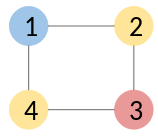
\includegraphics[height=2.1cm,width=2.3cm]{images/graphs/exampleGraph2.png}
  \caption{graph P}
  \label{fig:exampleGraph2}
\end{minipage}%
\begin{minipage}[t]{.4\textwidth}
  \centering
  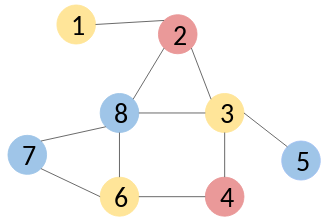
\includegraphics[height=3.4cm,width=5cm]{images/graphs/exampleGraph.png}
  \caption{graph T}
  \label{fig:exampleGraph}
\end{minipage}%
\begin{minipage}[t]{.3\textwidth}
  \centering
  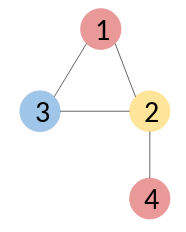
\includegraphics[height=3.4cm,width=3cm]{images/graphs/smalltarget.png}
  \caption{graph T1}
  \label{fig:exampleGraph}
\end{minipage}%
\caption{Instances of subgraph isomorphism problem (SIP)}
\label{fig:SIP}
\end{figure}

%% induced : if edge in p, then edge in t, but if edge not in p then edge not in t
%% non-induced: if edge in p, then edge in t
\subsection{The Subgraph Isomorphism Problem}
A \emph{subgraph} of \emph{G} is a graph \emph{H} whose vertices and edges are subsets of the vertices and edges of \emph{G} and the labeling on the vertices is preserved.

A \emph{non-induced subgraph isomorphism} is an injective mapping \emph{i} : \emph{P} $\rightarrow$ \emph{T} from a graph \emph{P} to a graph \emph{T} that preserves adjacency and labeling on vertices. That is, if \emph{v} $\sim_{P}$ \emph{w}, then \emph{i(v)} $\sim_{T}$ \emph{i(w)} and if L(\emph{P}, \emph{v}) = l, then L(\emph{T}, \emph{i(v)}) = l. The \emph{non-induced subgraph isomorphism problem} (SIP) is to find such a mapping from a given graph \emph{P}, called a pattern, to a given graph \emph{T} referred to as a target. The \emph{induced} SIP additionally requires that if \emph{v} $\nsim_{P}$ \emph{w} then \emph{i(v)} $\nsim_{T}$ \emph{i(w)}. In this work, we discuss only the non-induced version. We say that an instance of SIP is \emph{satisfiable} (SAT) if such a mapping \emph{i} exists. Otherwise, the instance is \emph{unsatisfiable} (UNSAT).

\begin{example}
\label{ex:sip}
Lets us consider the two graphs in Figure \ref{fig:SIP}. The SIP instance between the pattern P (in the left-hand side of the Figure) and the target T (the graph in the middle of the Figure) is SAT- the mapping from P to T maps vertex 1 to vertex 8, vertex 2 to vertex 3, vertex 3 to vertex 4 and vertex 4 to vertex 6.
\end{example}

% \gls{sip} is NP-complete, however there exist a number of different approaches to solve it, some of which are ... 
There are various existing algorithms for the subgraph isomorphism problem \cite{vf2,Solnon:2010,CP2015,Larrosa:2002,Bonnici:2013,Zampelli:2010,nauty}. More thorough analysis of the problem and discussion on existing work is presented in Section \ref{sec:sipalgos}.

\subsection{The Filter-Verification Paradigm}
A \emph{database} \emph{D} is a set of target graphs. A set of pattern graphs is called a \emph{query set} or \emph{queries}, is denoted by \emph{Q}. Let \emph{S} be the Cartesian product of \emph{Q} and \emph{D}. \emph{Subgraph query processing} is the process of solving the \gls{sip} for every pair in \emph{S}.

\begin{example}
\label{ex:pathIndexing}
Let us consider again Figure \ref{fig:SIP} and assume that graph P (in the left-hand side) is the query set \emph{Q}, and graphs T (in the middle) and T1 (in the right-hand side) represent the graph database \emph{D}. Then, subgraph query processing would solve the SIP for instances (P, T) and (P, T1), where the former instance will be determined as SAT (Example \ref{ex:sip}) and the latter as UNSAT (there is no valid mapping from P to T1). 
\end{example}

%% todo: cite the np-complete part
Another way of processing queries is the \emph{filter-verification framework}, which consists of two steps. The \emph{filter} step tries to prune targets that can not be matched to a given query. The set of targets left after this step formes the set of \emph{candidates}, denoted as $\fancyC_{p}$, where $\fancyC_{p}$ $\subseteq$ T. The following \textit{verification} step then performs \gls{sip} for every pair (G$_{p}$,$\fancyC_{G_{p}}$) $\in$ P $\times$ $\fancyC_p$. The usage of the filter-verification paradigm is motivated by the fact that subgraph isomorphism is NP-complete and reducing the number of \gls{sip} calls by discarding targets that are \gls{unsat} for a given pattern during the filtering step and performing \gls{sip} using the limited set of candidates would yield to significant performance improvement \cite{ctindex,foteini}.

%%% TODO: move all definitions about filter-verif here

There are various subgraph query processing algorithms based on the filter-verification framework \cite{ctindex,gcode,graphgrepsx,tree+delta>=graph,GRAPES}. This approach is discussed in more detail in Chapter \ref{ch:existingWork}, where more definitions and annotations are introduced in Section \ref{sec:filterVerificationParadigm} followed by analysis of related work in Section \ref{sec:ctindex}.

% how do we build the database index?
% using a pre-built index of the database, denoted as $\fancyI_{T}$

% what is a candidate set?
% graph index, features, ...
% what is false-positive? what is false-negative, why it can't exist?

% TODO
\subsection{Filtering}
This step consists of building an index of the database and then rejecting for verification with the query targets that can be proved not to contain the query. The process of rejecting/pruning uses the data stored in the index for the particular target and the characteristics of the query. The details follow below.

\subsubsection{Database Index}
An \emph{index} of a database D, denoted as $\fancyI_{D}$ is a collection of data, often stored in a file, that contains characteristics of the graphs in D, also known as \emph{features}. Features can be represented by paths, subtrees, cycles, or subgraphs. They are computed for every graph in the database. The index is independent of the queries so that it can be computed once and then reused for multiple queries as long as there is no change in the database. The process of computing the features of the graph to store them in the index is called \emph{feature extraction}.

\begin{example}
\label{ex:index}
Let us have a database consisting of the graph G$_{t}$ displayed on Figure \ref{fig:exampleGraph}. In this example, we want to compute the index of G$_{t}$ using paths up to maximum length 2 as features and store each unique path as a string containing the labels of the vertices in the path. Each vertex in G$_{t}$ is labeled in yellow(Y), blue(B) or red(R).

An example feature extraction algorithm will derive the following paths:
B, Y, R, B-B, B-Y, R-Y, B-R \footnote{Note that the representation of some of the paths is not unique, as G$_{t}$ is undirected. For example, path B-Y is equivalent to path Y-B. In such cases, one can impose constraints on the ordering of the paths to avoid storing repetitive features in the index.}. These paths will then be stored in the index of G$_{t}$ and used further in the filtering process to check whether G$_{t}$ could be rejected for verification with a given query.
\end{example}

Computing the database index is the process is very expensive in terms of running time and data storage. However, the cost of building such structure is compensated by the fact that it can be reused and that it is query independent.

\subsubsection{Candidate Set}
The candidate set of a database D and query graph G$_{p}$, denoted as $\fancyC_{p}$ is a set of graphs that contain all features in G$_{p}$. $\fancyC_{p}$ is derived using $\fancyI_{D}$ and $\fancyF_{G_{p}}$, where $\fancyF_{G_{p}}$ contains all features in G$_{p}$, computed using the same algorithm that computed $\fancyI_{D}$. Note that unlikely $\fancyI_{D}$, $\fancyF_{G_{p}}$ is not reused\footnote{It could be useful to store the query features if large proportion the queries received were repetitive. In such cases, one could incrementally build a second index of the features. We do not know whether this has been tried so far. This can be an area of further investigation in the future.}.

The purpose of filtering is to derive as small candidate set as possible in order to limit the number calls to a subgraph isomorphism algorithm during verification. Note that $\fancyC_{p}$ $\subseteq$ D. The worst case scenario is when $\fancyC_{p}$ = D, which means that filtering did not manage to prune any target graphs in the database.

\begin{example}
Let us extend Example \ref{ex:index} by introducing a query, which is the graph G$_{p}$ on Figure \ref{fig:exampleGraph2}. Let us use the same characteristics as features as the ones used in Example \ref{ex:index}. Then, $\fancyF_{G_{p}}$ = B, Y, R, B-Y, R-Y and G$_{t}$. Therefore, $\fancyC_{G_{p}}$ = \{G$_{t}$\}, because all features in G$_{p}$ are contained by G$_{t}$.
\end{example}

\subsection{Verification}
Verification is the process of applying a subgraph isomorphism problem (\gls{sip}) algorithm on every pair (G$_{p}$,t) of graphs, where p is the query and t is the target, t $\in$ $\fancyC_{G_{p}}$. The aim of verification is to return the number of graphs in D that contain G$_{p}$. All targets that do not contain the pattern, but were not rejected during the filtering step, are called \emph{false-positives}. One wants to construct a filtering technique that admits as low number of false-positives as possible. The number of false-positives is often used as a measure of effectiveness of the filtering method\cite{foteini}.

Most of the subgraph query processing methods that apply the filter-verification paradigm are mainly focused on improving the filtering stage, while reusing the same algorithm, known as VF2, for verification \cite{foteini}. 
It is claimed that VF2 is ``state of the art''\cite{ctindex}. However, this is not the case (\cite{Solnon:2010, Larrosa:2002, Bonnici:2013, Zampelli:2010, CP2015}, Chapter \ref{ch:evaluation}). The subgraph isomorphism tests are reported as ``too time consuming''\cite{foteini} and this is explained by the nature of the complexity of the subgraph isomorphism problem\footnote{This problem is proved is NP-Complete by Stephen A. Cook in 1971 \cite{Cook:1971}}\cite{ctindex,foteini,freqStructBasedIndexing}. One can see that the reason for the reported low verification performance for some instances could be due to the poor choice of a \gls{sip} algorithm. This is further investigated and discussed later in this work. 6  

\section{Aims and Motivations}
The subgraph isomorphism problem involves finding a pattern graph inside a target graph, where a graph is a structure that represents schemaless data such as proteins, chemical compounds, and XML documents. Subgraph isomorphism has a wide variety of applications in many fields. For instance, finding the best treatment to fight a particular cancer involves screening a patient's tumor to search for particular set of biomarkers \cite{nature:2015}. Such tasks involve repeatedly examining a large number of graphs, typically stored in a database, comparing each of them with a pattern.

%% patrick and ciaran's sip paper:
Applications include bioinformatics\cite{Bonnici:2013}, chemistry\cite{Regin:1995}, computer vision\cite{Damiand:2011,Solnon:2015}, law enforcement\cite{Coffman:2004}, model checking\cite{Calder:2015} and pattern recognition\cite{Conte:2004}.
%    Many substructure-searching problems call for repeatedly examining a large number of molecules (typically stored in a database), comparing each with a pattern. In such situations, it pays to spend some time "up front," storing the answers to specific questions for each structure in the database. Subsequent searches of the database use these pre-computed answers to vastly improve search time; the up-front computation time is paid back quickly as repeated searches are performed.
%        \begin{itemize}
%            \item graphs are widely used nowadays to represent data
%            \item the graph containment problem is widely addressed in many areas of science: genetics, chemistry, XML documents, images, fraud detection and prevention (there was an article in nature about this)
%        \end{itemize}
        
%        In the core of many graph-related applications, lies a common and critical problem: \textit{how to efficiently process graph queries and retrieve related graphs}. In some cases, the success of an application directly relies on the efficiency of the query processing system.  
        
%        Applications:
%        \begin{itemize}
%        \item genome sequencing: find mutations responsible for rare diseases -- nature vol 527 no 7576
%        \item treating diseases like cancer: screen a patient's tumor for a set of biomarkers to choose the best treatment to fight the particular cancer -- nature vol 527 no 7578
%        \end{itemize}

The remaining of this work is organised as follows. Section \ref{sec:graphTheory} contains terminology, definitions and notation used throughout this work. Chapter 2 presents review and analysis of existing approaches to solve the problem and properties of 4 real datasets used for testing and evaluation. An implementation and empirical analysis of two graph indexing and filtering methods is presented in Chapter 3. Chapter 4 describes a new approach to solve the problem, called Light Filters. The evaluation of Light Filters and analysis of the hardness of satisfiable and unsatisfiable subgraph isomorphism instances in the datasets are presented in Chapter 5. Chapter 6 provides a summary of this work and suggestions how to extend it in the future. 


%%%%%%%%%%%%%%%%%%%%%%%%% CHAPTER 2 %%%%%%%%%%%%%%%%%%%%%%%%%%%%
\chapter{Review of existing work}
\label{ch:existingWork}
\section{The nature of the problem}


%%%% datasets
\section{Datasets}
\label{sec:datasets}

This Section includes the specifications and the nature of the four real datasets used for performance study of existing work in Section \ref{subsec:ctindexEval} and for evaluation in Section \ref{ch:evaluation}. The datasets are obtained from \cite{datasets}. Many related research publications use some of them to assess the performance of their developed subgraph query processing methods \cite{ctindex, gcode, graphgrepsx, tree+delta>=graph, GRAPES, lindex, foteini}. Therefore, running our experiments on these datasets makes our results easier to compare to existing work. Description of each dataset and its specifications are explained below.

All four datasets consist of undirected labeled graphs, as defined in \ref{sec:graphTheory}, that may contain cycles. Each dataset has a set of target graphs, also called a database, and a set of query graphs. Every graph and every vertex within every graph have a unique id.

Aids is the standard database of the Antiviral Screen dataset of the National Cancer Insitute. The database contains the topological structure of 40,000 chemical compounds, represented as graphs. The number of vertices varies from 4 to 245. The graphs in this dataset are small and barely connected \ref{table:datasets}. Pcms contains 200 contact maps that represent relationships among amino acids. The graphs here are small and dense. Pdbs consists of 600 target graphs, which represent proteins. It contains larger graphs, each of them contains between 1,683 and 7,979 vertices. The last dataset is ppigo and it has a database that consists of 20 protein interaction networks, where networks belong to species.

The specifications of each dataset is shown in Table \ref{table:datasets}. One can see that the pcms dataset is very dense, as the average vertex degree is 23.01. Pdbs and aids are very sparse with average vertex degree of about 2. The dataset with lowest number of edges per graph is aids (46.95) and the dataset with largest number of edges per graph on average is ppigo (4,942).

Table \ref{table:dataSAT} shows the number and percent of \gls{sat} \gls{sip} instances for each dataset. For instance, pdbs consists of large number of \gls{sat} problems (77.22\%), whereas aids is the dataset with highest percent of \gls{unsat} problems (91.33\%).

\begin{table}
\centering
        \renewcommand{\arraystretch}{1.4}% Spread rows out...
        \begin{tabular}{l|r|r|r|r|}
\cline{2-5}
& \textbf{aids} & \textbf{pcms} & \textbf{pdbs} & \textbf{ppigo} \\
\cline{1-5}
\multicolumn{1}{|l|}{\# graphs}  & 40,000 & 200	& 600   & 20 \\
\hline
\multicolumn{1}{|l|}{\# disconnected graphs} & 3,157 & 200 & 360 & 20 \\
\hline
\multicolumn{1}{|l|}{\# unique labels} & 62 & 21 & 10 & 46 \\
\hline
\multicolumn{1}{|l|}{\# vertices on average} & 45 & 377 & 2,939 & 4,942 \\
\hline
\multicolumn{1}{|l|}{\# edges on average} & 46.95 & 4,340 & 3,064 & 4,942 \\
\hline
\multicolumn{1}{|l|}{average density} & 0.0475 & 0.0612 & 0.0007 & 0.0022 \\
\hline
\multicolumn{1}{|l|}{average vertex degree} & 2.09 & 23.01 & 2.06 & 10.87 \\
\hline
\multicolumn{1}{|l|}{\# labels on average} & 4.4 & 18.9 & 6.4 & 28.5 \\
\hline
\end{tabular}
\caption{Characteristics of the datasets}
\label{table:datasets}
\end{table}

\begin{table}
\centering
        \renewcommand{\arraystretch}{1.5}% Spread rows out...
        \begin{tabular}{l|r|r|r|r|r|r|r|r|}
            \cline{2-9}
            &
             \multicolumn{2}{c}{\textbf{AIDS}} & 
             \multicolumn{2}{|c}{\textbf{PCMS}} & 
             \multicolumn{2}{|c|}{\textbf{PDBS}} & 
             \multicolumn{2}{c|}{\textbf{PPIGO}} \\
            \cline{2-9}
              & number  & percent & number & percent & number & percent & number & percent \\
              \hline
            \multicolumn{1}{|l|}{\textbf{all SIP calls}}  &240,000   &100 &1,800 &100 &3,600 &100 &100 &100 \\
            \multicolumn{1}{|l|}{\textbf{SAT SIP calls}}  &20,816 &8.67 &592 &32.8 &2,780 &77.22 &61 &61 \\
            \multicolumn{1}{|l|}{\textbf{UNSAT SIP calls}} &219,184 &91.33 &1,208 &67.2 &820 &22.78 &39 &39 \\
            \hline
        \end{tabular}
        \caption{Number of SIP instances for each dataset and how many of them are SAT and UNSAT}
        \label{table:dataSAT}
    \end{table}


\section{Filter-Verification paradigm}
\label{sec:filterVerificationParadigm}
This Section gives an overview of already existing algorithms based on the filter-verification paradigm, defined in Section \ref{sec:theory}.

\subsection{Existing Filtering Techniques}
\label{subse:existingFVtechniques}

This Section discusses some of the existing filtering algorithms with respect to feature extraction and choice of features.

There are two types of feature extraction techniques, known as graph mining and exhaustive feature enumeration. \emph{Graph mining} techniques (\cite{freqStructBasedIndexing,fg-index,closure-tree,cp-index,lindex,tree+delta>=graph,treepi}) store the frequent features with high enough discriminative ratio in the database. A feature is \emph{frequent} if its support ratio is higher or equal to a certain algorithm-specific threshold value. The support ratio of a feature is defined as the percentage of graphs in the database containing it. The \emph{discriminative ratio} of a feature is a metric that characterizes the filtering power of the particular feature compared to other features. There is no universal formula to calculate the discriminative ratio of a feature, every technique employs a different calculation method.

\emph{Exhaustive feature enumeration} techniques (\cite{graphgrepsx,ctindex,anotherindex,gcode}) store in the index all features of every graph in the database, regardless of their importance.  

Choosing a feature extraction method often depends on the type of datasets one has to work with. For instance, graph mining techniques are inefficient when the data in the database is frequently being changed. When frequently inserting and deleting graphs in the database, the discriminative ratio of the indexes features may change so that it makes the index outdated. Consequently, the index becomes less reusable and thus the total execution time of subgraph query processing is highly increased.  Moreover, graph-mining techniques take longer time to built the database index \cite{foteini}.

One of the advantages of graph mining techniques is that they require much less storage space than exhaustive feature enumeration algorithms, as one does not need to store all features of all graphs. This lowers the storage space requirements and makes the process of constructing the candidate set faster, as less number of target features have to be compared against the query features.

There are various types of structures that can be used as features. Paths (\cite{graphgrepsx,GRAPES}), trees (\cite{closure-tree,treepi,ctindex}), subgraphs (\cite{fg-index,anotherindex,cp-index,lindex,tree+delta>=graph}) of the targets or all of them combined (\cite{ctindex,tree+delta>=graph}) can be extracted from the database graphs and stored in the index. Features can be derived based on the neighbours of each graph vertex \cite{gcode}. The choice of features influences the filtering performance and it is often a trade off in terms of time and filtering strength. This is further investigated in Section \ref{subsec:ctindexEval}, where we report on performance results obtained from an indexing method that uses a combination of paths, trees and graph cycles as features. A detailed review of this method is presented in the next Section.
%%%%%%%%%%%%%%%%%%%%%%%%%%%%%%%%%%%%%%%%%%%%%%%%%%%%%%%%%%%%%%%%%%%%%%%%%%
%%                               CT-Index                               
%%%%%%%%%%%%%%%%%%%%%%%%%%%%%%%%%%%%%%%%%%%%%%%%%%%%%%%%%%%%%%%%%%%%%%%%%%
\section{CT-Index}
\label{sec:ctindex}

CT-Index is an existing subgraph query processing approach that employs the filter-verification paradigm\cite{ctindex}. This method supports undirected graphs with edge and vertex labels and also wild card patterns. Although not explicitly stated in \cite{ctindex}, CT-Index addresses the non-induced subgraph isomorphism problem defined in Section \ref{sec:theory}. In this Section, we introduce and discuss the filtering algorithm and analyze its complexity in Section \ref{subsec:ctindexF}. Section \ref{subsec:ctindexV} explains the verification algorithm. Also presented is a complexity analysis of the algorithms used by CT-Index and an empirical study of its performance (using an open-source Java implementation) in Section \ref{subsec:ctindexEval}.

\subsection{Filtering}
\label{subsec:ctindexF}
During the filtering step, the features of all graphs in the target data set are extracted and saved to a file, i.e. the target index ($\fancyI_{T}$). $\fancyI_{T}$ is used to filter out target graphs (G$_{t}$) that cannot contain the pattern (G$_{p}$). Features are specific subgraphs used to classify graphs, and are stored as hash-key fingerprints. Features may be paths, subtrees or cycles of bounded length. Since vertices and edges may contain labels, these features can be viewed as strings from a specified alphabet (where the alphabet is the labels). In \cite{ctindex} it is stated that the reason for using \glspl{tree} and cycles (as well as paths) is that ``trees capture additional structural information" and cycles ``represent the distinct characteristic of graphs, often neglected when using only trees as features".

Although the time complexity of computing all features of a graph is not reported, it can be derived as follows. To extract a subtree of graph $G$ with e$_{max}$ number of edges, one starts with initially empty tree and repeatedly adds edges to extend the vertices that are in the current tree via the recursive function ExtendTree. We write F for the set of every edge e$_{uv}$ $\in$ G with vertices \textit{u} $\in$ G and \textit{v} $\in$ G, such that one of them (say, \textit{u}) is part of the current tree and the other (say, \textit{v}) is not. If we have \textit{n} number of vertices in the current tree, each with degree \textit{d}, then the size of F is at most n(d - 1). ExtendTree adds an edge specified as parameter to the current tree, generates F and makes a recursive call for every e$_{uv}$ $\in$ $F$, until the tree reaches size e$_{max}$.

%%% todo for the big O
In the start of the \gls{tree} extraction when adding the first edge to the empty tree, the vertices on both ends of the edge are also added as part of the tree. Therefore, the size of $F$ initially is 2.(d-1). After every recursive call, one more vertex is added to the tree, which introduces (d-1) new edges. That makes a total of e$_{max}$ + 1 vertices that will be added to the tree and (e$_{max}$ + 1)(d - 1) visited edges. Consequently, the complexity of extracting tree features is $\mathcal{O}(|e|(e_{max} + 1)(d - 1))$. From this formula one can see that the number of edges in the graph has significant impact on the performance of the algorithm. When increasing the graph density, the algorithm will have slower performance, caused by the degree of each vertex and the total number of edges, which both will increase.

CT-Index computes a unique representation of each distinct feature, its \emph{\gls{canonicalform}}, and stores its string encoding in $\fancyI_{T}$. Thus, the equality of two features can be checked by testing the equality of their canonical forms. The canonical label of a tree feature is computed as follows: (1) find the root node \emph{r} of the tree, (2) impose a unique ordering of the children of each node. Step (1) is computed by repeatedly removing all leaf nodes of a tree until a single node or two adjacent nodes remain. In the first case, \emph{r} is the last node left. In the second case the edge connecting the two remaining nodes are removed to obtain two trees, each with one of the remaining nodes as a root.
Step (2) is based on the ordering of edge and node labels. For each node \textit{p} that is a parent of nodes \textit{u} and \textit{v}, deciding whether \textit{u} is before \textit{v} depends first on the labels of the edges e$_{pu}$ and e$_{pv}$, then on the labels of \textit{u} and \textit{v} and finally on the subtrees of \textit{u} and \textit{v}. A bottom-up approach is used (i.e. start with the nodes in the lowest level and move up towards the root) to compute this.

%%%% complexity of canonical label algorithm %%%%
Although not stated in \cite{ctindex} the complexity of their canonical labeling can be derived as follows. Step (1) is $\mathcal{O}(n)$, where $n$ is the number of nodes in the tree, as one needs to visit each node before removing it. The complexity of step (2) is as follows. We write $|p|$ for the number of interior nodes in the trees, which is equal to $n$ minus the number of leaf nodes. Step (2) visits a node, then visits its parent, and for every child of the parent node checks whether it should be first or second in the canonical label, using the vertex and edge labels conditions described above. This is repeated for every node in the tree up to the root. Therefore, the complexity of step (2) is $\mathcal{O}(|p|.|c|^{2})$, where $|c|$ denotes the number of children of a parent.

%%% 
In \cite{ctindex} it is claimed that step (2) is not linear time but is tolerable because ``... the trees occurring as features usually are small and vertex and edge labels are diverse and hence the order can be solved quickly". Therefore, we might assume that CT-Index is designed to support only specific types of data sets. Therefore one could expect poor performance for data sets with less label diversity and with big trees as features. More specifically, as e$_{max}$ increases, or average degree increases, so too does the cost of step (2), and performance suffers (we conduct experiments to test this hypothesis in Section \ref{subsec:ctindexEval}).

\subsubsection{Fingerprints}

%%%% hash-key fingerprints %%%%
CT-Index uses a storage technique called \emph{hash-key fingerprint} to capture the features in the graph. A separate fingerprint is computed from the canonical labels for each graph in the database. A fingerprint is an array of bits and denotes whether a particular feature occurs in the graph or not. As there is no predefined set of possible features for each graph, reserving one bit for each feature in the feature set is considered infeasible\footnote{However, due to the restricted alphabet of labels it may be possible to enumerate all possible features thus avoiding some of the pitfalls of hashing, such as collisions and sensitivity to hash table size.}. A \gls{hashfunction} maps extracted features to bit positions.
CT-Index is not the first indexing algorithm to employ fingerprints as a storage technique. The chemical information system called Thor and developed by Daylight \cite{fingerprints} is an example of an information processing system that uses bit arrays to store the features of the graphs.

%%%
Information on the implementation of the hash function is not specified in the paper. Depending on the quality of the hash function, the size of the bitset and the size of the fingerprint, collisions may occur, i.e. different features may map to the same bitset position, introducing false-positives. The \cite{ctindex} paper briefly discusses some optimization techniques that could be used to minimize the influence of collisions, but it is unclear whether CT-Index employs them. 
It is stated that ``... the loss of information caused by the use of hash-key fingerprints seems to be justifiable by the compact nature and convenient processing of bit arrays as long as the amount of false positives does not increase significantly due to collisions".

Collisions can occur also if the size of the fingerprint is too small for the particular data, i.e. there is bigger number of features than the number of spaces in the array to store them. However, making the fingerprint size too big introduces additional overhead by requiring more memory storage space that is not used. The paper does not specify the hash function used or how to decide on the size of bitsets (feature hash tables). 

%%%% advantages %%%%
The main advantage of hashing the features and storing them in arrays is that this makes certain operations much cheaper. For example, checking whether a pattern fingerprint is included in a target fingerprint involves inexpensive bit operations. In particular, one only needs to compute a bitwise AND-operation with the two fingerprints to determine if features in the pattern exist within the target. If this test returns false then the target cannot be a candidate for that pattern. However, if it returns true then the target \emph{may} be a candidate and subgraph isomorphism must be verified.

%%%%%%%%%%%%%%%%%%%%%%%%%%%%%%%%% 
\subsection{Verification}
\label{subsec:ctindexV}

The verification step checks all candidates computed in the filtering step via a subgraph isomorphism test. A backtracking algorithm \cite{backtracking-algorithms}, similar to VF2 \cite{vf2} with additional heuristics, is used.  This test is theoretically NP-Complete, and is avoided as far as possible via the filtering process. CT-Index is not alone in using (essentially) the VF2 algorithm.
For example it is used in GraphGrepSX \cite{graphgrepsx}, gCode \cite{gcode} and Tree+$\Delta$ \cite{tree+delta>=graph}. Most papers claim that VF2 is ``state of the art".  However, this is not the case (\cite{Solnon:2010,Larrosa:2002,Bonnici:2013,Zampelli:2010,CP2015}.
VF2 has been shown to perform erratically and poorly \cite{CP2015}. Therefore we might summarize CT-Index architecture as using a potentially expensive indexing and filtering stage in order to minimize the computational cost of using an outdated \gls{sip} algorithm.

%%%%%%%%%%%%%%%%%%%%%%%%%%%%%%%%%
\subsection{Performance}
\label{subsec:ctindexEval}

There is an existing work, where several well-established subgraph query processing techniques as well as CT-Index are evaluated \cite{foteini}. The experiments are conducted on the four datasets described in Section \ref{sec:datasets} using the default input parameters for each of the compared techniques. CT-Index requires five integers as an input, specified in the following order:
\begin{enumerate}
\item Fingerprint size. This indicates the number of bits allowed to store the features of each graph in the index. The specified fingerprint size must be equal to 2$^{n}$ for some integer n.
\item Maximum path length. Indicates the maximum length of a path that is allowed to be extracted. If we specify -1, then no paths are extracted.
\item Maximum subtree length. Same as 2, but for subtrees.
\item Maximum cycle length. Same as 2 and 3, but for cycles.
\end{enumerate}
%The main conclusions that were made after the experiments are as follows.
%\begin{enumerate}
%\item Datasets with increased number of distinct labels are easier and faster to filter and verify.
%\item The size of the query affects performance, especially when the datasets contain graphs of high density.
%\item CT-Index has relatively small index size, compared to other indexing techniques.
%\item There is no universal subgraph query processing method that is guaranteed to be the best one across different datasets.
%\end{enumerate}

The default input parameters of CT-Index are $<$4096, -1, 4, 4 $>$ \cite{ctindex, foteini}. No information on why exactly these parameters should be used is given. For each of the four datasets, the indexing algorithm is run, putting a time limit of 8 hours\footnote{When the algorithm did not finish it execution within the time limit, the authors waited for more than 24 hours, but to no avail.}. The obtained results are presented in four Diagrams, showing filtering time, index size, verification time and false positive ratio (FP ratio). The FP ratio is calculated using formula (2.1) and its purpose is to indicate how many of the \gls{unsat} instances are filtered without using a \gls{sip} algorithm. \textit{$|A\{p\}|$} denotes the number of \gls{sat} instances for a pattern p $\in$ P and \textit{$|\fancyC\{p\}|$} is the cardinality of the candidate set for p.
\begin{equation}
\label{eq:fpratio}
FP Ratio = \frac{1}{|P|} \sum_{p \in P} \frac{|\fancyC\{p\}| - |A\{p\}|}{|\fancyC\{p\}|}
\end{equation}

One can notice that when the value of \textit{$|A\{p\}|$} becomes closer to the value of \textit{$|\fancyC\{p\}|$} (filtering has managed to discard most of the \gls{unsat} instances), the FP ratio approaches 0. Whenever there is a big difference between \textit{$|\fancyC\{p\}|$} and \textit{$|A\{p\}|$} (filtering did not discard many \gls{unsat} instances, the size of the candidate set is close to the size of the database)  the formula approaches 1. We can deduce that the closer to 1 this formula is, the less successful filtering was. Similarly, when the formula approaches 0, this indicates high filtering performance.
 
The results obtained by \cite{foteini} using these parameters for each dataset are as follows.
\begin{itemize}
\item For datasets ``pcm'' and ``ppigo'', CT-Index never manages to complete execution of the filtering step. Therefore, no verification is done.
\item For the ``aids'' dataset, CT-Index performs best. Filtering takes about 80 seconds and verification: about 0.7 seconds. The FP ratio is 0.8.
\item CT-Index takes about 9,000 seconds for filtering graphs in ``pdbs'' and about 1 second to execute the verification step. The FP ratio is 0.2.
\end{itemize}

We decided to conduct experiments to investigate in more depth the performance of the algorithms implemented in CT-Index depending on the input parameters. We used an open source java implementation of CT-Index written by its authors and we ran the software with the ``aids'' dataset using alternative to the default set of parameters. For our experiments, we chose a fixed size of parameter set\footnote{This was done due to the large number of possible input values.} the purpose of which is to identify how the change of one parameter changes the performance of the algorithms implemented in CT-Index. As in \cite{foteini}, we measured the filtering and verification time, the FP ratio using formula (2.1) and calculated the total time, that is the sum of the filtering and the verification time. For the size of the fingerprints (2$^{n}$ for some integer \textit{n}), we varied \textit{n} from 0 to 16. Note that when n is 0, no index can be created (all features of every graph have to be stored in a bitset of size 1) and verification is computed for every pair (G$_{p}$, G$_{t}$) $\in$ P$x$. The values of path, subtree and cycle maximum length are a permutation of combination of -1 and 5. Here, -1 tells us how much the effective rate of filtering drops when a feature is switched off, and 5 shows the performance of filtering when the feature is on (i.e -1 and 5 play the role of binary to indicate for each feature that it is either off or on). For every \textit{n}, we executed the algorithm with all permutations of every combination of assignment of -1 and 5.

Table \ref{table:runningTime} shows a selection of our results that aids to illustrate best the change of performance depending on the input parameters. The first 10 rows show the changes in running time and FP-ratio depending on the size of the fingerprints. The values of all parameters are fixed. As expected, the FP ratio goes down with the increase of the fingerprint size. We also notice significant decrease in the verification running time when we allow bigger bitset size. The reason for these results is the fact that the number of collisions when hashing the features to places in the bitset is lower when the bitset has bigger size. Then, more targets can be rejected during filtering and less number of \gls{sip} tests have to be computed during verification.

%%%% big table with ct-index running times and results on the AIDS dataset %%
\newcommand\TstrutT{\rule{0pt}{2.6ex}}         % = `top' strut
\newcommand\Bstrut{\rule[-1ex]{0pt}{0pt}} 

\begin{table}
%\begin{minipage}
\begin{center}
\renewcommand{\arraystretch}{1.2}% Spread rows out...
\begin{tabular}{ |c|r|r|r|r|r|}\hline
 Row \# & Input & Filtering T[sec]& Verification T[sec]& Total T[sec] & FP Ratio\\
 \hline
  1 & 1 5 \,\,5 \,\,5 & 108.934  & 67.395 & 176.329 & 0.913 \\
 \hline
  2 & 64 5 \,\,5 \,\,5 & 110.797 & 59.622 & 170.419 & 0.85 \\
 \hline
  3 & 128 5 \,\,5 \,\,5 & 110.9 & 31.711 & 142.611 & 0.87 \\
 \hline
  4 & 256 5 \,\,5 \,\,5 & 104.586 & 22.373 & 126.959 & 0.81 \\
 \hline
  5 & 512 5 \,\,5 \,\,5 & 104.883 & 17.008 & 121.891 & 0.69 \\
 \hline
  6 & 1024 5 \,\,5 \,\,5 & 112.132 & 15.477 & 127.609 & 0.64 \\
 \hline
  7 & 2048 5 \,\,5 \,\,5 & 107.024 & 14.693 & 121.717 & 0.63 \\
 \hline
  8 & 4096 5 \,\,5 \,\,5 & 106.136 & 13.006 & 119.142 & 0.60 \\
 \hline
  9 & 8192 5 \,\,5 \,\,5 & 107.625 & 12.337 & 119.962 & 0.62 \\
 \hline
  10 & 16384 5 \,\,5 \,\,5 & 107.991 & 14.083 & 122.074 & 0.61 \\
 \hline
  11 & 4096 5 \,\,5 -1 & 105.441 & 12.926 & 118.367 & 0.62 \\
 \hline
  12 & 4096 5 -1 \,\,5 & 39.743 & 32.068 & 71.811 & 0.88 \\
 \hline
  13 & 4096 -1 \,\,5 -1 & 81.826 & 12.785 & 94.611 & 0.62 \\
 \hline
  14 & 4096 -1 -1 \,\,5 & 6.234 & 61.346 & 67.580 & 0.913 \\
 \hline 
  15 & 4096 -1 \,5 \,5  & 82.376 & 5.896 & 88.272 & 0.62\\ 
 \hline
  16 & 4096 \,\,5 -1 -1 & 37.621  & 7.929 & 45.550 & 0.88 \\ 
 \hline 
\end{tabular}
\caption{CT-Index: Running time and results depending on the specified parameters}
\label{table:runningTime}
\end{center}
%\end{minipage}
\end{table}
%%%

The last 7 rows of Table \ref{table:runningTime} show the performance of CT-Index depending on the other 3 parameters. The input with the worst verification run time is in row 14. No target was rejected during the filtering stage for each of the patterns, as indicated by the high FP ratio value. This data shows that extracting only cycles as features is not effective in pruning and it is almost equivalent to not having an index structure at all. A reason for this can be that the graphs in the datasets don`t' have many cycles.

Comparing the results from rows 8 and 15, one can see that extracting paths and subtrees as features for this dataset gives worse performance in both filtering and verification steps. The reason for this could be that subtrees and cycles are descriptive enough to be used as the only types of features.

Using only paths as features is the option that shows best performance (row 16). Subtree extraction for this dataset takes about 60 seconds more, it gives better filtering ratio, however slightly worse verification run time(rows 16 and 11). From this we can see that the algorithm for subtree extraction significantly lowers the filtering run time, as derived during the empirical analysis in \ref{subsec:ctindexF}. One can reach the same conclusion when comparing rows 15 and 16. The options in row 15 give better performance during verification time, but they result in more than twice slower filtering time.

We tried running similar experiments with the other datasets discussed in \ref{sec:datasets}. However, as also observed in \cite{foteini}, most of the experiments finished computation within matter of days.


\section{Subgraph Isomorphism with Constraint Programming}
\label{sec:sipalgos}
% todo: patrick's algorithm is not solved with constraint programming
Subgraph isomorphism problem (\gls{sip}) can be solved using tools of constraints programming. This constraint-based search approach dates back to works by Ullmann\cite{Ullmann:1976}. We can model it as a CSP by creating a variable \emph{x$_{u}$} for every vertex \emph{u} in the pattern graph. The domain of \emph{x$_{u}$} denoted as \emph{D$_{u}$} is the set of vertices in the target graph. A global \emph{AllDiff} constraint \cite{Regin:1994} ensures that no two pattern vertices are matched with the same vertex from the target. In addition, a binary constraint is introduced for each edge in the pattern to guarantee that every edge in the pattern graph is associated to an edge in the target graph. The set of solution of SIP is equal to the set of all valid assignments of target vertices to pattern vertices. The initial size of the search space is the Cartesian product of the initial domains of all variables. 

There are various pieces of existing work that employ this model \cite{Solnon:2010, Ullmann:1976, Regin:1995, Larrosa:2002, Solnon:2010a, CP2015}, where the exact constraints and the level of filtering varies. The algorithm presented in \cite{CP2015} is bit- and thread parallel and introduces the use of supplemental graphs to create implied constraints. It is discussed in more detail in Section \ref{sec:sippatrick}.% In \cite{Solnon:2010}, an iterative labeling is introduced to associate a global label for each vertex based on its neighbourhood. This algorithm is discussed in Section \ref{sec:sipchristine}.

\subsection{Partick and Ciaran's paper}
\label{sec:sippatrick}
%% what SIP, what types of graphs?
The paper discusses the non-induced version of the subgraph isomorphism problem for finite, undirected graphs that do not have multiple edges between pairs of vertices, but may have loops. Although the algorithm does not consider labels, it can be easily adjusted to take into account labeled vertices and/or edges by adding additional constraints. In fact, adding labeling support would make the algorithm faster, as follows from a result proved in \cite{Ciaran:2016}. Unlikely most recent work in subgraph isomorphism\cite{Solnon:2010a,SND}, this algorithm replaces strong inference with cheaper techniques and shows that they can be beneficial. The algorithm exploits parallelism for both pre-processing and search and introduces a novel usage of backjumping that does not need maintaining conflict sets. 

%% graph representation
The algorithm uses bitset encodings: graphs are represented as bit sets, each pattern vertex has a domain which is a bit set. This representation allows for fast execution of operations. For instance, the neighbourhood intersections discussed shortly are bitwise-and operations, the unions of domains used during alldifferent propagation and nogood values discovered during search are computed using bitwise-or operations, and cardinality checks involve computing the Hamming weight (also known as population count) of the set \cite{Reed:1954}, which is a single instruction in modern CPUs \cite{CP2015}.  

%% explain supplemental graphs
The supplemental graph G$^{[c,l]}$ is a graph that has at least \emph{c}
number of paths of length exactly \emph{l} between two vertices \emph{v} and \emph{w} in G\cite{CP2015}. Supplemental graphs are based on the idea that \emph{i}: \emph{P} $\rightarrow$ \emph{T} is a subgraph isomorphism with target \emph{T} and pattern \emph{P}, then F(\emph{i}): F(\emph{P}) $\rightarrow$ F(\emph{T}) is a subgraph isomorphism for certain functions F. Supplemental graph pairs are constructed from the pattern and the target with bound on the path distance 3\footnote{The bound is chosen after an observation that distances greater than 3 rarely give additional filtering power and their construction is computationally very expensive \cite{CP2015}}. The intuition behind their usage is to put a restriction that vertices of distance \emph{x} apart must be mapped to vertices that are within distance \emph{x}. This also implies that adjacent vertices in the pattern must be mapped to adjacent vertices in the target. These restrictions are put on top of the search during the initialization of domains in order to perform initial filtering at the top of the search.

The initial filtering on top of the search also checks for compatibility of neighbourhood degree sequences of the pattern and target vertices, based on the fact that a vertex \emph{v} can only be mapped to a vertex \emph{w} if the sequence consisting of the degrees of every neighbour of \emph{w} is bigger or equal to the sequence consisting of the degrees of every neighbour of \emph{v} \cite{Solnon:2010}. Neighbourhood degree sequence compatibility was introduced by \cite{Solnon:2010} and is used in the Light filters approach introduced later in this work in Chapter \ref{ch:sip1}. 

%% explain search
The algorithm employs a recursive search procedure that repeatedly picks a variable with the smallest domain to branch on, breaking ties on descending static degree in the original pattern graph. The values of the domain of each variable are ordered by descending static degree in the target graph. If the assigned value to a variable is in conflict with the current partial solution or does not obey certain constraints, then the search returns a nogood set of variables. In such case, the algorithm can perform a variation of conflict directed backjumping \cite{Prosser:1993} without explicitly maintaining conflict sets. On success of value assignment of a variable, the algorithm updates the partical solution and makes recursive call until every variable is assigned (success) or no solution is proved to exist. 

%% explain the counting based alldifferent
A variable assignment algorithm is called every time a variable \emph{v} is to be given a value \emph{e} from its domain \emph{D$_{v}$}. The algorithm assigns \emph{e} to \emph{v} and then infers which values may be eliminated from the remaining domains. It removes \emph{e} from the domains of all other variables and eliminates any detected \glspl{hallset} from future variables\footnote{The algorithm may fail to identify some Hall sets if the initial ordering of domains is imperfect. However, it gives big pay off in terms of running time, as validated experimentally in the paper}, thus detecting that an assignment is impossible even if values remain in each variable`s domain.

%% explain the parallelism bit
The SIP algorithm achieves \gls{simd}-like parallelism from the bitset encodings. The algorithm also allows for parallel supplemental graphs construction, neighbourhood degree sequence calculation, graph construction and domain initialization. In addition, the subtrees created by recursive calls made during search can be explored in parallel by multiple threads using early diversity work-stealing approach, where a single thread always preserves the sequential search order, finding states of the search space that are to be explored. The rest of the threads take work from the main thread, trying to steal early in the search tree, because value-ordering heuristics are expected to be weakest early in the search \cite{Harvey:1995}.

%% evaluation and performance
Both the sequential and the threaded version of the algorithm was compared with an implementation of SND \cite{SND}, LAD\cite{Solnon:2010a} and VF2\cite{vf2}. The properties of the hardware, implementation-specific details, the nature of the datasets used in the experiments and the results from the evaluation are presented in the paper\cite{CP2015}. Below are highlights of the results obtained after the experiments:
\begin{itemize}
\item The algorithm is the single best among the evaluated approaches for non-trivial instances. VF2 is stronger on trivial instances. The reason for this the time needed to instantiate domains, generate supplemental graphs and perform the inference on top of the search. These results show that there is no single algorithm that performs best on all instances and suggests for taking more flexible future approach that allows for instance-specific configuration. For example, for trivial problems one may not need to create supplemental graphs.
\item Except at very low sequential runtimes, parallelism results in general improvement of speed. For exceptionally hard satisfiable instances, parallelism results to superlinear speedup. This shows that the early work stealing approach is able to recover from early mistakes of value ordering heuristic choices by avoiding strong commitment to such choices.
\item Backjumping always either pays for itself or gives slight improvement. For some instances, that constitute of highly structured data, it makes an improvement of several orders of magnitude.
\item The last part of the 
\end{itemize}

%%%%%%%%%%%%%%%%%% the path-based indexes %%%%%%%%%%%%%%%%%%%%
\chapter{Framework for graph indexing and filtering}
%%%%%%%%%%%%%%%%%%%%%%%%%%%%%%%%%%%%%%%%%%%%%%%%%%%%%%%%%%%%%%
This Chapter describes a subgraph-query filtering and indexing framework designed and implemented in Java. The framework implements the first stage of the filtering-verification paradigm with a choice of two feature enumeration and candidates extraction techniques: Path Index(PI) and Path-Subtree Index(PSI). Given two sets of graphs: one with patterns and the other one with targets(a.k.a database), the framework computes their indices and generates a candidate set for subgraph isomorphism, which is a subset of the database. In the next sections, we present the design and implementation of every component of the framework and comment on its complexity. Section \ref{sec:graph-representation} presents the choice of graph representation. Section \ref{sec:pathsExtraction} explains the paths extraction algorithm, a procedure based on \gls{dfs} with bound on the path length. Section \ref{sec:PIandPSI} describes PI and PSI and finally Section \ref{sec:performance} we comment on the performance of the framework and give suggestions to improve its efficiency.

\section{Graph representation}
\label{sec:graph-representation}
Graphs are  represented with a Java class \emph{Graph} that has an integer id and a collection of objects of type \emph{Vertex} as fields. A Vertex has an id, a label and a list of edges that connect it to its neighbours. The number of edges a Vertex has equal to its degree. An Edge object has a label and a destination Vertex as fields. As the graphs we are working with are not directed, two Edge objects are created to represent an edge. The first object has one of the vertices as destination Vertex and then added in the list of edges of the other Vertex: the source Vertex. The second edge object will have the source Vertex of the first edge object as destination Vertex and included in the list of edges of the destination Vertex of the first edge object, which will be its source Vertex. The label of both edge objects will be the same.

\section{Paths Extraction}
\label{sec:pathsExtraction}
A path is a sequence of distinct vertices, such that each successive pair of vertices are adjacent. A path can also be from a vertex to itself, in which case the first and the last vertices in the sequence are the same. Path extraction is referred to the process of generating all paths up to a given length l$_{max}$ in a graph G. For every vertex \emph{v} in G, we execute a recursive \gls{dfs} algorithm with a bound on the size of the stack of maximum number of vertices l$_{max}$. We output the sequence of vertices currently stored in the stack after each recursive call. Every generated sequence is then fed into the \ref{alg:outputPath} procedure to derive the p-feature and store it in the index.

Algorithm \ref{alg:generatePath} describes our approach. Before generatePath procedure is called, an empty stack \emph{s} is initialized (line 3). The stack is used for storing the sequence of vertices generated during \gls{dfs} procedure. Procedure generatePath ( \textrm{Algorithm \ref{alg:generatePath}}) takes all vertices in the target graph and l$_{max}$ as parameters. It calls procedure dfsBounded for every vertex in the list as starting vertex (line 5). The start vertex is also pushed on the stack (line 4), as it is part of the path that is to be generated.

Algorithm \ref{alg:dfsBounded} performs a \gls{dfs} with bound path length. Given a starting vertex \emph{v}, l$_{max}$ and stack s, Algorithm \ref{alg:dfsBounded} iterates through all neighbours of \emph{v}, adding each neighbour \emph{n} to the stack (line 10) and calling dfsBounded with \emph{n} as a starting vertex (line 11). At each call of dfsBounded, the current sequence of vertices in the stack is passed to procedure computeFeature (Algorithm \ref{alg:outputPath}) until all vertices reachable by the start vertex within distance l$_{max}$ are visited.

%%% proper path extraction algorithm
\begin{algorithm}
\centering
\caption{Paths extraction}
\label{alg:generatePath}
\begin{algorithmic}[1]
\Procedure{generatePath }{vertices, l$_{max}$}
\For{v in vertices}
	\State s $\gets$ init \Comment{\textit{initialize the stack}}
	\State push v on top of s
	\State \Call{dfsBounded}{v, l$_{max}$, s}
\EndFor
\EndProcedure
\end{algorithmic}
\end{algorithm}
%%% end of algorithm

%%% generatepath inner algorithm
\begin{algorithm}
\centering
\caption{Depth First Search of bound length}
\label{alg:dfsBounded}
\begin{algorithmic}[1]
\Procedure{dfsBounded }{v, l$_{max}$, s}
\If{s $\leq$ l$_{max}$}
\State newPath  $\gets$ s  \Comment{\textit{new path of size up to l$_{max}$ is found}}
\State \Call{getPath}{newPath}
\EndIf
\If{s == l$_{max}$}
\State s.pop()
\EndIf
\For{neighbour of v}
\If{neighbour not in s}
\State s.push(neighbour)
\State \Call{dfsBounded}{neighbour, l$_{max}$, s} \Comment{\textit{recursive call}}
\EndIf
\EndFor
\If{s is full} \Comment{\textit{all neighbours of node are on the stack}}
\State s.pop()
\EndIf
\EndProcedure
\end{algorithmic}
\end{algorithm}
%%% end of algorithm
%%% TODO check this complexity 
The complexity of dfsBounded is derived as follows. Algorithm \ref{alg:outputPath} iterates through each vertex in the graph, calling the dfsBounded procedure. The number of calls to dfsBounded from this Algorithm is equal to the order of the graph, say \emph{n}. Let us denote the degree of a vertex as \emph{d}. Then, dfsBounded will generate d$^{l_{max}-1}$ paths. This will result to \emph{d + d$^{2}$ + \ldots d$^{l_{max}-1}$} calls to dfsBounded in total. Therefore, the overall cost of extracting all paths in a graph of maximum length l$_{max}$ is $\mathcal{O}(n(d + d^{2} + \ldots d^{l_{max}-1}))$.

%%% TODO move this to a different section
%The filtering stage of the CT-Index algorithm reviewed in Section \ref{sec:ctindex} is used as a benchmark for the algorithms described here. 
%   The correctness of the results is checked comparing the answers obtained from CT-Index. We implemented a class called \textit{Verify} that checks whether the resulting candidate set after each query execution contains the answers of subgraph isomorphism. \textit{Verify} was very useful for discovering a lot of bugs during the software development process.

\section{Indexing and candidates extraction algorithms}
\label{sec:PIandPSI}
The rest of the subgraph query filtering process is carried out by using two algorithms: Path Index (PI) and Path-Subtree Index (PSI). PSI and PI employ different feature representation and candidates extraction algorithms, which are explained below.

%%%%%%%%%%%%%%%%%%%%%%%%%%%%%%%
\subsection{Path Index}
\label{sec:pi}
This Section presents PI: a technique to compute features of a graph commonly used in many filtering algorithms \cite{graphgrepsx}. Below we describe the features calculation and candidate extraction algorithms employed in PI.

\subsubsection{Features}
\label{sec:pifeatures}
PI computes the features stored in the index using the paths extracted during the path extraction procedure outlined in Section \ref{sec:pathsExtraction}. To store a path in $\fancyI_{D}$, we compute its unique string representation, referred to as \emph{p-feature}. The procedure to derive p-features and store them in $\fancyI_{D}$ is the following.
\begin{enumerate}
\item Given a sequence of vertices v$_{seq}$ (i.e. a path), replace each vertex in v$_{seq}$ with its label to obtain its \emph{p-feature}.
\item Reverse the sequence v$_{seq}$ to obtain v$_{seq}^{\prime}$.
\item Calculate \emph{p-feature}$^{\prime}$, that is the unique string representation of v$_{seq}^{\prime}$.
\item If not added previously, store in $\fancyI_{D}$ the lexicographically smaller of the two string representations (i.e. \emph{p-feature}$^{\prime}$ or \emph{p-feature}).
\end{enumerate}

The complexity of each of the four steps of the p-feature computation and storage is the following. Step 1 involves iterating through the sequence of vertices, that is at most $l_{max}$ elements. Accessing the label of each vertex is a constant time operation, therefore the complexity of Step 1 is $\mathcal{O}(l_{max})$. The complexity of Step 2 and Step 3 is $\mathcal{O}(l_{max})$. Step 4 has $\mathcal{O}(p)$ worst case complexity, where p is the current size of the index of the current graph being indexed. Note that as the index grows larger and larger, the cost of adding new p-features increases.

\begin{example}
Figure \ref{C2H4-1} represents a graph G with 6 vertices, each with an id: a number from 1 to 6, and a label: either yellow(Y) or blue(B). The sequence of vertices $<$1, 5, 6$>$ is a valid path, because every pair of consecutive vertices in the sequence are neighbours in G. Executing Step 1 of the procedure explained above results in obtaining the p-feature ``Y-B-B''. After computing Step 2 and 3, we derive the p-feature of the reversed sequence equal to ``B-B-Y''. We store the string ``B-B-Y'' in $\fancyI_{D}$, because it is lexicographically smaller than ``Y-B-B''.
\end{example}

The path extraction algorithm will encounter both v$_{seq}^{\prime}$ and v$_{seq}$ throughout its execution, but only one p-feature to represent both of them will be stored in the index. Storing the p-feature of both of them would be redundant, because the graphs we work with are undirected. Therefore, choosing to store only one of them (in this case the lexicographically smaller one) limits the size of the index by half.

%% TODO: prove this
\begin{theorem}
Let us have two paths: v$_{seq}$ and v$_{seq}^{\prime}$ in an undirected graph G, such that v$_{seq}^{\prime}$ is the reverse of v$_{seq}$. We can represent v$_{seq}$ and v$_{seq}^{\prime}$ using one p-feature without loosing structural information about G. 
\end{theorem}

\begin{proof}
The correctness of this statement follows from the fact that G is undirected. 
\end{proof}

%%%
\begin{figure}
\centering
\begin{minipage}[t]{.5\textwidth}
  \centering
  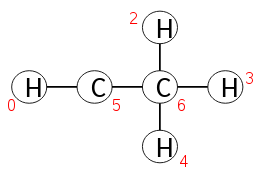
\includegraphics[height=3.3cm,width=4.4cm]{images/graphs/C2H4-1.png}
  \caption{Graph G}
  \label{C2H4-1}
\end{minipage}
\end{figure}
%%

\subsubsection{Implementation}
\label{pi:featuresImpl}
Algorithm \ref{alg:outputPath} describes the implementation of Steps 1-4 described above. Given a sequence of vertices \emph{vseq} as parameter, the procedure computes the \emph{p-feature} (line 2) and \emph{p-feature}$^{\prime}$ (lines 3, 4) and stores the lexicographically smaller variant in the index.

%%% proper output path algorithm
\begin{algorithm}
\centering
\caption{Compute p-features procedure}
\label{alg:outputPath}
\begin{algorithmic}[1]
\Procedure{computeFeature }{vseq}
\State pfeature $\gets$ vseq.toString() \Comment{\textit{returns a string of the labels of the nodes in vseq}}
\State rseq $\gets$ vseq.reverse() \Comment{\textit{reverse the order of nodes in vseq}}
\State pfeature$^{\prime}$ $\gets$ rseq.toString() \Comment{\textit{returns a string of the labels of the nodes in rseq}}
\If {pfeature$^{\prime}$ $<$ pfeature}
\State pfeature $\gets$ pfeature$^{\prime}$ \Comment{\textit{put to index the lexicographically smaller string}}
\EndIf
\If {pfeature not in $\fancyI_{D}$}
\State add pfeature to $\fancyI_{D}$
\EndIf
\EndProcedure
\end{algorithmic}
\end{algorithm}
%%% end of algorithm

\subsubsection{Candidates Extraction}
%for each path in the pattern index: check whether there exists the same path in the target index. Output the ids of all targets that contain all paths of the pattern.
The process of computing the set of candidates for subgraph isomorphism test with the pattern is referred to as candidate extraction. Algorithm \ref{alg:piCandidatesExtraction} shows the procedure. It returns a list of the ids of all graphs in the database that contain all p-features of the pattern graph \emph{p}. Algorithm \ref{alg:piCandidatesExtraction} iterates once through all graphs in the database (line 3) and for each target checks whether it contains all p-features of the pattern (lines 5, 6, 7). Let the number of targets be \emph{n}, the size of the pattern be \emph{p$_{i}$} and the average size of a target graph index be \emph{t$_{i}$}. Then the time complexity is equal to $\mathcal{O}(n. p_{i}. t_{i})$.

\begin{algorithm}
\centering
\caption{Candidates Extraction Procedure}
\label{alg:piCandidatesExtraction}
\begin{algorithmic}[1]
\Procedure{candidatesExtractor }{$\fancyI_{G_{p}}$, $\fancyI_{G_{t}}$}
\State{candidates $\gets$ new ArrayList$<>$()}
\For{ Graph t : targets}
	\State{flag $\gets$ true}
	\For{pfeature : $\fancyI_{G_{p}}$}
    	\If{\textbf{not} \Call{contains }{ t.index, pfeature}} \Comment{\textit{check whether pfeature is contained in the index of t}}
        	\State{flag $\gets$ false; break}
        \EndIf
	\EndFor
    \If{flag}
    	candidates.add(t.id)
    \EndIf
\EndFor
\State{\Return{candidates}}
\EndProcedure
\end{algorithmic}
\end{algorithm}

%%%%%%%%%%%%%%%%%%%%%%%%%%%%%%%%%
\subsection{Path-Subtree Index}
\label{path-subtree-index}
Path-Subtree Index (PSI) is a novel indexing technique based on the notion of vertex neighbourhood label, somewhat similar to the labeling approach used for solving the subgraph isomorphism problem employed by \cite{Solnon:2010}. This Section presents the algorithm for computing the p-features of paths and the candidates extraction approach employed in PSI. We prove that PSI has greater filtering power than PI.

\subsubsection{Features}
The difference between PSI and PI is the approach of computing the unique string representation (p-feature) of paths. The difference lies in the labeling employed by PSI: it is based on the neighbourhood label of a vertex. Below we discuss the notion of vertex neighbourhood label and the procedure of computing p-features.

\subsubsection{Vertex Neighbourhood Label}

The term \emph{neighborhood label (n-label)} refers to a specific label that is computed for each vertex in the graph using the labels of the vertices in its neighbourhood. The n-label of a vertex \emph{v} with label \emph{l} is a string composed of the labels of its neighbours and \emph{l} ordered in lexicographically increasing order, starting always with \emph{l}.

\begin{example}
\label{ex:nlabel}
Figure \ref{C2H4-1} represents a graph with 6 vertices with ids from 1 to 6. Each vertex is labeled either in yellow (Y) or in blue (B), as shown in the Figure. The n-label of vertex 6 is ``BBYYY'', as it is its label is B, it has 4 neighbours, 3 of them with label Y and one with label B. Similarly, the n-label of vertex 5 is ``BBY'', and the n-label of vertices 1, 2, 3 and 4 is equal to ``YB''.
\end{example}

\begin{enumerate}
\item Given a sequence of vertices v$_{seq}$, replace each vertex in v$_{seq}$ with its \emph{neighbourhood label (n-label)} to obtain the p-feature of v$_{seq}$.
\item Reverse the sequence v$_{seq}$ to obtain v$_{seq}^{\prime}$.
\item Calculate \emph{p-feature}$^{\prime}$, that is the unique string representation of v$_{seq}^{\prime}$.
\item If not added previously, store in $\fancyI_{D}$ the lexicographically smaller of the two string representations (i.e. \emph{p-feature}$^{\prime}$ or \emph{p-feature}).
\end{enumerate}

\subsubsection{Implementation}

The toString method used in Algorithm \ref{alg:outputPath} is modified to take a bit as an input, which constructs a p-feature using the n-labels of the vertices of the bit is set or returns a p-feature composed of the labels of the vertices otherwise.

One can see that the difference between the features representation and computation between PI and PSI lies only in Step 1. The algorithm to implement the features representation and storage is almost the same as the one for PI with (Algorithm \ref{alg:outputPath}). The only difference is the modification of the toString() method (line 2,4) to output the n-labels or the labels of the vertices in the sequence depending on the value of a bit given as an input parameter. The p-features are constructed using labels of vertices if the bit is set to false or using the n-labels otherwise. The n-labels of the vertices in each graph are computed prior to the invocation of Algorithm \ref{alg:outputPath}, as explained below. Thus there is no additional time complexity to the features representation and storage algorithm used in PI.

Computing the n-label of a vertex is done after all the graphs from the input files are read and initialized. Additional field called n-label of type String and methods to compute it are added to the Vertex class. Algorithm \ref{alg:nlabel} shows our approach. It is executed for every vertex in every target. For every vertex, we compute a sequence of labels of its neighbours ordered lexicographically. The complexity of insertion sort is $\mathcal{O}(n^{2})$ \cite{backtracking-algorithms} and therefore the overall complexity of running Algorithm \ref{alg:nlabel} is $\mathcal{O}(d.n^{2})$, where \emph{d} denotes the average degree of a vertex.
 
%%% n-label algorithm
\begin{algorithm}
\centering
\caption{Set n-label procedure}
\label{alg:nlabel}
\begin{algorithmic}[1]
\Procedure{setNlabel }{}
\State{nlabel $\gets$ ``''}
\For{Edge e : this.edges}
\State u $\gets$ e.dstVertex
\State \Call{insertionSort }{nlabel, u.label} \Comment{\textit{Insert u`s' label in n-label in lexicographically increasing order}}
\EndFor
\EndProcedure
\State{nlabel $\gets$ label + nlabel} \Comment{\textit{append the label of the vertex to its n-label}}
\end{algorithmic}
\end{algorithm}
%%% end of algorithm

\subsubsection{Candidates extraction}
\label{pi:candExtr}
This Section describes how the set of candidate graphs for a \gls{sip} test with the pattern is formed, using the database index $\fancyI_{D}$ and the set of features of the pattern $\fancyI_{G_{p}}$.

The method to extract the candidate set is the same as the one shown in Algorithm \ref{alg:piCandidatesExtraction}. The only change is in the implementation of the contains procedure (Algorithm \ref{alg:piCandidatesExtraction} line 6). Instead of checking whether there exists a feature in the target index \emph{Tindex} that is identical to a given pattern feature \emph{pf}, we check whether the following two conditions are met:
\begin{enumerate}
\item The label of a vertex in i$^{th}$ position in the target path is equal to the label of a vertex in i$^{th}$ position in the pattern path.
\item The nlabel of a vertex in  i$^{th}$ position in the target path contains the nlabel of a vertex in i$^{th}$ position in the pattern path.
\end{enumerate}

The first condition is equivalent to the filtering procedure employed by PI: we check for compatibility using only the labels. The purpose of the second condition is to verify that the neighbourhood of each pattern vertex can be matched to a neighbourhood of a vertex in the target.

Algorithm \ref{alg:psicandidatesExtraction} illustrates the implementation of the contains procedure. For every path in the target index, it calls Algorithm \ref{alg:psicontainsFeature} to check that the two conditions discussed above are met (Algorithm \ref{alg:psicandidatesExtraction} line 3). If condition 1 (Algorithm \ref{alg:psicontainsFeature} line 2) is met, then procedure containsLabel checks whether condition 2 is satisfied (Algorithm \ref{alg:psicontainsFeature} line 8). Procedure containsLabel takes two nlabels as arguments and returns true if the second nlabel is contained in the first nlabel or false otherwise.
%%% 
\begin{algorithm}
\centering
\caption{Contains procedure}
\label{alg:psicandidatesExtraction}
\begin{algorithmic}[1]
\Procedure{contains }{Tindex, patPath} \Comment{\textit{Tindex is the target index, patPath is path in the pattern index}}
\For{tarPath : Tindex}
	\If{\Call{containsFeature}{tarPath, patPath}}
    \State{\Return{true}}
    \EndIf
\EndFor
\State{\Return{false}}
\EndProcedure
\end{algorithmic}
\end{algorithm}

\begin{algorithm}
\centering
\caption{containsFeature procedure}
\label{alg:psicontainsFeature}
\begin{algorithmic}[1]
\Procedure{containsFeature}{tarPath, patPath}
\If{tarPath.length $<$ patPath.length} \Return{false} \Comment{\textit{if tarPath is shorter than patPath, then it can`t contain it}}
\EndIf
\If{label of each vertex in tarPath \textbf{not equal} label of each vertex in patPath} \Comment{\textit{equivalent to PI filter}}
	\State{\Return{false}}
\EndIf
\For{i in range(0, tarPath.size())} \Comment{\textit{for i$^{th}$ nlabel in tarf, check that it contains the i$^{th}$ nlabel in patPath}}
    \If{\textbf{not} \Call{containsLabel}{tarPath.get(i), patPath.get(i)}}
        \State{\Return{false}}
    \EndIf
\EndFor
\State{\Return{true}}
\EndProcedure
\end{algorithmic}
\end{algorithm}

Algorithm \ref{alg:psicandidatesExtraction} involves visiting each path in the index of a single target, calling Algorithm \ref{alg:psicontainsFeature} (line 3), which then visits at most all characters that form a given nlabel. Therefore, the overall complexity of Algorithm \ref{alg:psicandidatesExtraction} is linear with the size of the input.

%%% WHY IS NEIGHBORHOOD METHOD BETTER? %%%
\begin{theorem}
\label{psiisbettertheorem}
Let $\fancyC_{PI}$ be the candidate set retrieved by PI and let $\fancyC_{PSI}$ be the candidate set obtained after running the framework using PSI. Then $\fancyC_{PSI}$ $\subseteq$ $\fancyC_{PI}$.
\end{theorem}

\begin{proof}
The first filtering condition implemented by Algorithm \ref{alg:psicontainsFeature} puts an upper bound on the size of $\fancyC_{PSI}$ to be at most $|\fancyC_{PI}|$ and condition 2 gives PSI additional filtering strength by requiring an existence of matching of the neighbourhood of each pattern vertex to a neighbourhood of a vertex in the target. Therefore $\fancyC_{PSI}$ $\subseteq$ $\fancyC_{PI}$. 
\end{proof}

\section{Running the framework}
To run the framework, the user specifies the names of the files containing all target and all pattern graphs, $l_{max}$ (the bound on the path length allowed to be extracted) and a bit denoting which indexing and candidates extraction technique the user wants to run. If the bit is 1, the framework will index the graphs using PSI, otherwise it will run PI. The source code can be downloaded from Github \cite{framework-github}.

\section{Performance analysis and suggestions for improvement}
\label{sec:performance}
%%% TODO: make some small experiments and put them in the appendix, then put a reference to the appendix here.
In this Section we discuss the performance of the framework using PI and PSI. Both of them were ran with the datasets described in Section \ref{sec:datasets} and their filtering strength and execution time was compared with CT-Index \cite{ctindex}, analyzed in Section \ref{sec:ctindex}. CT-Index results are also used as a benchmark for correctness of the implemented algorithms. We outline the strengths and weaknesses of PI and PSI and give suggestions for improvement.

Let us denote the index and the candidate set obtained after running the framework using PI as $\fancyI_{PI}$ and $\fancyC_{PI}$ respectively, and the index and the candidate set obtained after running the framework using PSI as $\fancyI_{PSI}$ and $\fancyC_{PSI}$. 

PSI requires significantly more storage space than PI. In particular, if we assume that the average vertex degree in the target database is \emph{d}, the p-feature of each path computed using PSI will be \emph{d} times bigger than the p-feature of the same path computed using PI due to the size of the nlabel of each vertex. Therefore, the size of $\fancyI_{PSI}$ is three times bigger than the size of $\fancyI_{PI}$.

Theorem \ref{psiisbettertheorem} states that the filtering performance of PSI is not worse than the filtering performance of PI. In practice, the size of $\fancyC_{PSI}$ is rarely close to the size of $\fancyC_{PI}$. In particular, when running the framework with the AIDS dataset (Section \ref{sec:datasets}) with maximum path length of 2, 3, 4 and 5, the size of $\fancyC_{PSI}$ was several times smaller than the size of $\fancyC_{PI}$. Moreover, setting the maximum path length bound to 5 removes 80\% of the unsatisfiable instances on average. This filtering result is not only better than PI, but it also outperforms CT-Index.

Both PI and PSI are much slower than CT-Index. In particular, increasing the maximum path length bound significantly increases the algorithms computation time. This stems from the fact that maximum path length makes great impact on the complexity of the path extraction algorithm and on the size of the index. PSI is slower than PI both during index computation and candidates extraction time. Looking at the difference in their time complexities, this result is not surprising.

The filtering power of PSI and PI does increase linearly when increasing the maximum path length bound. There exists a bound \emph{m} on the maximum path length after which there is almost no filtering gain, but only significantly increased computation and storage overhead. The value of \emph{m} is usually smaller for PSI than for PI. For instance, when PSI is ran with instances from the AIDS dataset, \emph{m} is equal to 5. This is the peak when the algorithm performs best. Any value larger than 5 results in much worse computation speed and almost unchanged filtering performance.

There are several ways in which the framework can be made more efficient. In the framework, the index of a database is the union of the indices of all targets. Naively, it does not take into an account the fact that a feature can be present in more than one graph. When working with datasets where the graphs are similarly structured like AIDS, removing repetitive features results in significant decrease of the index size. The following strategies can be employed to decrease the size of the index without lowering its filtering capability.

We can represent the index using a \gls{tree} data structure similar to \gls{sufftree} \cite{weiner:1973} that stores all extracted features from the database as strings and number of leaf nodes of the tree denotes the number of features. The representation of strings in the tree is the same as the representation employed by \glspl{sufftree} except from the construction of leaf nodes and the feature suffixes insertion. Each leaf node is a list of the ids of all graphs that contain the corresponding feature. We insert the full feature without inserting its suffixes. This is because each label/nlabel part of a feature is a feature on its own and it will be extracted from the path extraction algorithm. Therefore, there is no need to insert unique termination character at the end of a feature, as it is done with \glspl{sufftree}. The tree can be built incrementally during features extraction in $\mathcal{O}(n.log(n))$ time on average, where \emph{n} is the length of the string that results when appending all features in the database, and worst-case time complexity $\mathcal{O}(n^{2})$. More efficient suffix tree construction algorithms exist \cite{weiner:1973, McCreight:1976, Ukkonen:1995} that could be adjusted to work for the tree. Searching for a feature \emph{F} of length \emph{m} in the suffix tree requires following a path from the root matching characters until reaching the leaf node and can be done in $\mathcal{0}(m)$ time. %Therefore, candidates extraction with pattern index with \emph{n$_{p}$} number of features of average length \emph{m$_{p}$} and target index with \emph{n$_{d}$} number of features of average length \emph{m$_{d}$} would take $\mathcal{O}(n)$ has time complexity $\mathcal{O}()$

%Alternative way is to represent the index as a dictionary. - having a dictionary structure to keep every feature and the number of times it occurs in the particular graph. Analyze what the complexity of this would be, would it be better and why.

%- the framework provides a functionality to save the index to a file and then reuse it from the file. In practice, the way the code works at the moment is to store the target index in memory. Experiments with the datasets used by big data research community were run on a simple machine and no memory overflow was encountered.

%- reduce the index size by employing the maximal features thing (cite needed papers --- graphgrepsx about the idea and the early IBM paper about the notion of descriptive feature).

% TODO: write that we can represent the graphs using bitset encodings. cite the papers cited by patrick and ciaran's sip paper.

%%%%%%%%%%%%%%%%%%%%%%%%%%%%%%%%%%%%%%%%%%%%%%%%%%%%%%%%%%%%%%%%%%%%%%%%%%%%
%%%------------------------------SIP Algorithms--------------------------%%%
%%%%%%%%%%%%%%%%%%%%%%%%%%%%%%%%%%%%%%%%%%%%%%%%%%%%%%%%%%%%%%%%%%%%%%%%%%%%

%% todo
%% remove sip0 and make sip1 be sip 0
%% make the graphs be in log scale
\chapter{Light Filters}
\label{ch:sip1}
This section describes the study of a simple subgraph isomorphism problem(\gls{sip}) algorithm, called SIP1, that implements a fast filter that does not employ an index structure.

Light Filters is an algorithm for subgraph query processing and it is based on a modified version of the filter-verification paradigm. Here, filtering and verification steps are applied separately for each \gls{sip} instance. This approach uses simple filtering tests that require much less computational effort (i.e. lighter filtering). More importance is placed on the quality of the \gls{sip} algorithm than on the filters, because the major computational effort goes for solving the non-filtered \gls{sip} instances. 

Algorithm \ref{algo:roughSIP} is a pseudocode of our method. Given a file with targets T and a file with patterns P, we first read in each graph (lines 2, 3). Filtering is performed for every (G$_{p}$, G$_{t}$) pair and if the instance is not rejected, a call to \gls{sip} algorithm is made (line 7). The filter step consists of 5 naive tests, performed before the call to SIP1. If the conditions of any of the tests are not met, search does not proceed and we consider this to be a \textit{trivial fail}. 

Each step of the Light Filters algorithm is explained thoroughly. First, we introduce the theory behind the trivial fails and their implementation in Section \ref{sec:trivialFails}. We then introduce the SIP algorithm called SIP1 and discuss its implementation in Section \ref{sec:sip1}. Evaluation of the light filters approach is described in Chapter \ref{ch:evaluation}.

%%% light filters sip algorithm
\begin{algorithm}
\centering
\caption{Light filters algorithm}
\label{algo:roughSIP}
\begin{algorithmic}[1]
\Procedure{Process }{File p, File t} \Comment{\textit{file with patterns and file with targets}}
\State T$_{list}$ $\gets$ read in all targets from file, initialize objects
\State P$_{list}$ $\gets$ read in all patterns from file, initialize objects
\For{G$_{p}$ in P$_{list}$}
	\For{G$_{t}$ in T$_{list}$}
		\If{!\Call{Filter }{G$_{p}$, G$_{t}$}} \Comment{\textit{If the instance is not rejected during filtering, perform verification}}
    		\State{\Call{SIP1}{G$_{p}$, G$_{t}$}}
    	\EndIf
    \EndFor
\EndFor
\EndProcedure
\end{algorithmic}
\end{algorithm}
%%%% end of algorithm

\section{Trivial Failures}
\label{sec:trivialFails}

This Section introduces the five trivial failure tests, implemented as part of the filtering stage of SIP1.

\subsection{Neighborhood Degree Sequence}
\label{sec:nds}
The neighbourhood degree sequence of G and the degree sequence of labels in G correspond to four of the trivial tests. Very similar approach of using the degree sequence of vertices to reject \gls{unsat} \gls{sip} instances is used in the filtering part of the algorithm presented in \cite{Solnon:2010}.
 
\begin{definition}[Label Degree Sequence]
The \textit{\gls{lds}} of \textit{l} $\in$ L$_{G}$, denoted as $\gls{lds}$(G, \textit{l}) is the non-increasingly ordered list of the degrees of all vertices in V$_{G}$ that have \textit{l} assigned as their label.    
\end{definition}

\begin{definition}[Neighborhood Degree Sequence]
The \textit{\gls{nds}} of G, written as $\gls{nds}$(G), is the list of tuples (\textit{l}, $\gls{nds}$(\textit{l})) for every \textit{l} $\in$ L$_{G}$.
\end{definition}

\begin{example}
Let us have a graph G with two labels: A and B, where \gls{lds}(A) = \{5, 4, 3, 2, 2\} and \gls{lds}(B) = \{4, 3, 3, 1\}. This shows us that the order of G is 9, where 4 vertices with degrees 4, 3, 3 and 1 are labeled as B and 5 vertices with degrees 5, 4, 3, 2 and 2 are labeled as A. Using \gls{lds}, we derive that \gls{nds}(G) = \{\{A, \{5, 4, 3, 2, 2\}\}, \{B, \{4, 3, 3, 1\}\}\}.
\end{example}

\begin{definition}[G$_{t}$ subsumes G$_{p}$]
\label{def:subsumes}
We say that G$_{t}$ subsumes G$_{p}$ if for each label l both in G$_{p}$ and G$_{t}$, the length of the \gls{lds}(l$\in G_{p}$) is smaller or equal to the length of \gls{lds}(l$\in G_{t}$), and the degree on i$^{th}$ position in \gls{lds}(l$\in G_{p}$) is less than or equal to \gls{lds}(l$\in G_{t}$) for each i between 0 and $|\gls{lds}(l\in G_{p})|$.
\end{definition}

The notion of \gls{nds} lets us define several simple tests for incompatibility between \gls{pattern} and \gls{target}, based on checking whether \gls{nds}(G$_{p}$) is a subset of \gls{nds}(G$_{t}$). \gls{nds}(G$_{p}$) $\subseteq$ \gls{nds}(G$_{t}$) if all following conditions are true:
\begin{enumerate}
\item the order of G$_{p}$ is less than or equal to the order of G$_{t}$
\item the number of unique labels in G$_{p}$ is less than or equal to the number of unique labels in G$_{t}$
\item every label in G$_{p}$ is also in G$_{t}$
\item G$_{t}$ subsumes G$_{p}$
\end{enumerate}

\begin{example}
Let us have \gls{nds}(G$_{p}$) = \{\{A, \{3, 2, 1\}\}, \{B, \{4\}\}\} and
\gls{nds}(G$_{t}$) = \{\{A, \{5, 4, 3, 2, 2\}\}, \{B, \{4, 3, 3, 1\}\}, \{C, \{5, 4, 2, 1\}\}\}.

In this example, \gls{nds}(G$_{p}$) is a subset of \gls{nds}(G$_{t}$), because each of the four conditions is true. In particular:
\begin{enumerate}
\item The order of G$_{p}$ (4) is less than the order of G$_{t}$ (13).
\item The number of unique labels in G$_{p}$ = 2 and the number of unique labels in G$_{t}$ is 3. 3 is clearly bigger than 2.
\item G$_{p}$ has labels A and B which are both in G$_{t}$.
\item The \gls{lds} of every label in G$_{p}$ is clearly contained in the \gls{lds} of the same label in G$_{t}$.
\end{enumerate}
\end{example} 

\begin{theorem}
\label{th:nds}
If \gls{nds}(G$_{p}$) $\nsubseteq$ \gls{nds}(G$_{t}$), then \gls{sip}(G$_{p}$, G$_{t}$) is \gls{unsat}.
\end{theorem}

\begin{proof}
Suppose that \gls{sip} (G$_{p}$, G$_{t}$) is \gls{sat} and that \gls{nds}(G$_{p}$) $\nsubseteq$ \gls{nds}(G$_{t}$). Then, at least one of the conditions for \gls{nds}(G$_{p}$) $\subseteq$ \gls{nds}(G$_{t}$) is not true.
\begin{enumerate}
\item Suppose that the first condition is false. Then, G$_{p}$ must have at least one vertex more than G$_{t}$, i.e. at least one vertex $\in$ G$_{p}$ will be unmatched. Therefore, \gls{sip} (G$_{p}$, G$_{t}$) is \gls{unsat} if the order of G$_{p}$ is bigger than the order of G$_{t}$ and we reach a contradiction. Therefore, this condition must always hold.
\item Suppose that the second condition is false so that there exists a label l$^{\prime}$ $\in$ L$_{G_{p}}$ with l$^{\prime}$ $\notin$ L$_{G_{t}}$. Therefore, there exists a vertex \textit{v} $\in$ G$_{p}$ that is assigned the label l$^{\prime}$ and there is no vertex in G$_{t}$ with label l$^{\prime}$. From this follows that \textit{v} can not be matched to any vertex in G$_{t}$ and \gls{sip}(G$_{p}$, G$_{t}$) is \gls{unsat}, which leads to a contradiction. Therefore, condition 2 must hold.
\item Suppose that the third condition is false. Then, there exists a label l$^{\prime}$ $\in$ L$_{G_{p}}$ and l$^{\prime}$ $\notin$ L$_{G_{t}}$. As proved before, this is a contradiction, therefore condition 3 must hold.
\item Suppose that previous three conditions hold and G$_{t}$ does not subsume G$_{p}$.

First, suppose that for each label l both in G$_{p}$ and G$_{t}$, the length of the \gls{lds}(l$\in G_{p}$) is smaller or equal to the length of \gls{lds}(l$\in G_{t}$). Then, there exists a degree value \textit{deg$_{pi}$} $\in$ \gls{lds}(l$\in G_{p}$) at position \textit{i} in the list for \textit{i} between 1 and $| \gls{lds}(l\in G_{p})|$ such that \textit{deg$_{pi}$} $>$ \textit{deg$_{ti}$}, where \textit{deg$_{ti}$} $\in$ \gls{lds}(l$\in G_{t}$). Then, there is a vertex \textit{v} $\in$ G$_{p}$ with label l and degree \textit{deg$_{pi}$} that will not be matched to any vertex in G$_{t}$. Therefore \gls{sip} (G$_{p}$, G$_{t}$) is \gls{unsat} which is a contradiction, therefore the degree of the \textit{i$^{th}$} element in \gls{lds} of each label in G$_{p}$ has to be smaller or equal to the degree of the \textit{i$^{th}$} element for the corresponding label in G$_{t}$ for every \textit{i} between 0 and the length of \gls{lds} of every label in G$_{p}$.

Second, suppose that there exists a label l both in G$_{p}$ and G$_{t}$ such that the length of the \gls{lds}(l$\in G_{p}$) is bigger than the length of \gls{lds}(l$\in G_{t}$). Then, the number of vertices with label l in G$_{p}$ is bigger than the number of vertices with label l in G$_{t}$ and it is impossible to match each vertex in G$_{p}$ to a different vertex in G$_{t}$ which leads to contradiction.

Therefore both conditions of subsumption must hold and G$_{t}$ subsumes G$_{p}$. This is a contradiction, therefore condition 4 must be true.
\end{enumerate} 

All four conditions must hold. It follows that \gls{nds}(G$_{p}$) $\subseteq$ \gls{nds}(G$_{t}$) which is a contradiction. Therefore, if \gls{nds}(G$_{p}$) $\subseteq$ \gls{nds}(G$_{t}$), then \gls{sip}(G$_{p}$, G$_{t}$) is \gls{unsat}.
\end{proof}

The four conditions for \gls{nds}(G$_{p}$) $\subseteq$ \gls{nds}(G$_{t}$) are the first four of the trivial failures added to SIP1, also displayed on Table \ref{table:failures}. Their implementation is discussed in Section \ref{sec:trivialFailsImplementation}.

\subsection{Domain wipe out}
\label{sec:domainWipeout}
This is the fifth of the trivial failures implemented as light filtering on top of the search. Every pattern vertex \textit{v} has a bitset domain \textit{dom$_{v}$}. The size of \textit{dom$_{v}$} is equal to the order of the target, where every bit corresponds to a vertex in the target. For every vertex \textit{w} $\in$ G$_{t}$, if L(\textit{w}) is equal to L(\textit{v}) and the degree of \textit{v} is smaller or equal to the degree of \textit{w}, we set the bit for \textit{w} in \textit{dom$_{v}$} to true, i.e. \textit{v} can be mapped to \textit{w}. Whenever no bit in \textit{dom$_{v}$} is set to 1, it means that no target vertex exists that can be mapped to \textit{v} i.e. no valid mapping from all vertices in G$_{p}$ to a different vertex in G$_{t}$ can exist and \gls{sip} (G$_{p}$, G$_{t}$) is \gls{unsat}. The algorithm returns false without proceeding to search.

Table \ref{table:failures} shows the trivial failures discussed. They are executed as tests in the same hierarchy as shown in the Table. The first four failures are namely the conditions for \gls{nds}(G$_{p}$) $\subseteq$ \gls{nds}(G$_{t}$). If either of these tests fails, then \gls{sip}(G$_{p}$, G$_{t}$) is \gls{unsat} (Theorem \ref{th:nds}).

\subsection{Order of Tests}

Tests follow a strict hierarchy, where test 1 performs the cheapest and most trivial task and test 5 is the most expensive and its filtering is based on the least trivial test. The cost of each test in terms of complexity is discussed in Section \ref{sec:trivialFailsImplementation}.

%%% todo: make a discussion about the dependency between these failures, i.e. what happens if we switch off one failure or not. Write an informal proof about it?

%\begin{itemize}
%\item Filter 2 and 3 filter differently. Ex: p = \{A,B,B,C\} and t=\{A,B,C\}. Test 2 passes, but test 3 fails
%\end{itemize}

%%%% table about failures %%%%
\begin{table}
\centering
\renewcommand{\arraystretch}{1.5}% Spread rows out...
\begin{tabular}{ >{\centering\bfseries}m{1in} >{\centering\arraybackslash}m{2.3in}} 
\toprule
  Trivial Fail & Meaning\\
\midrule
 \textbf{1} & G$_{t}$.order $\geq$ G$_{p}$.order\\
 \rowcolor{Gray}
 \textbf{2} & G$_{t}$ unique labels $\geq$ G$_{p}$ unique labels\\
 \textbf{3} & G$_{p}$ labels $\subseteq$ G$_{t}$ labels\\
 \rowcolor{Gray}
 \textbf{4} & G$_{t}$ subsumes G$_{p}$\\
 \textbf{5} & \textit{dom$_{v}$}, \textit{v} $\in$ G$_{p}$ not empty\\
 \bottomrule
\end{tabular}
\caption{Specification of the measured failure types}
\label{table:failures}
\end{table}        
%%%%

\subsection{Implementation}
\label{sec:trivialFailsImplementation}
Algorithm \ref{algo:filters} describes the implementation of the 5 trivial failures from Table \ref{table:failures} as part of the filtering stage. Procedure ``filter'' is executed for every \gls{sip} instance before the verification stage. If any of the if statements (lines 2, 4, 6, 8 and 17) is false, the procedure returns false and the verification for the corresponding instance is not executed. Otherwise, if all 5 tests are true, the procedure makes a call to SIP1, i.e proceeds to the verification step. Pseudocode for SIP1 is shown in Algorithm $say where$ and discussed in the next Section.

%% comment on the expensiveness of each trivial failure
Failures 1 and 2 are the fastest: each of them takes time $\mathcal{O}(1)$ to compute. For failure 1, one needs only to return the sizes of the number of vertices in G$_{p}$ and in G$_{t}$. For failure 2, for every graph G, we have an array that stores all unique labels that occur in G. The size of this array is known after the graph is read from the file. To check whether test 2 is true, one needs to compare the size of the labels array d$_{p}$ of G$_{p}$ with the size of the labels array d$_{t}$ of G$_{t}$. Finding the values of d$_{t}$ and d$_{p}$ takes time $\mathcal{O}(1)$.

Failures 3 and 4 have slower running time. For every label l $\in$ G$_{p}$, failure 3 occurs if l is not a label in G$_{t}$. Checking whether l is a label in G$_{t}$ involves iterating over the labels in G$_{t}$, which is of time $\mathcal{O}(d_{t})$ worst case, if l is the last label in G$_{t}$ or it is not present. Therefore, the overall complexity of failure 3 is $\mathcal{O}(d_{p}.d_{t})$. Algorithm \ref{algo:subsumes} shows the pseudo code for the ``subsumes'' procedure. Its complexity is $\mathcal{O}(plds)$, where plds is the \gls{lds} of label \textit{l} $\in$ G$_{p}$. Therefore, the overall complexity of failure 4 is $\mathcal{O}(plds.d_{p})$.

Failure 5 is the most expensive one. It takes time $\mathcal{O}(m.n)$, where n is the order of G$_{p}$ and m is the order of G$_{t}$. Algorithm \ref{algo:filters} has to visit each vertex \textit{v} $\in$ G$_{p}$, initialize dom$_{v}$ and for every \textit{w} $\in$ G$_{t}$, check whether \textit{w} can be mapped to \textit{v}. The two checks (line 13) take time $\mathcal{O}(1)$.

%% failures algorithm
\begin{algorithm}
\centering
\caption{Lights Filters}
\label{algo:filters}
\begin{algorithmic}[1]
\Procedure{Filter }{G$_{p}$, G$_{t}$}
\If {\textbf{not} G$_{t}$.order $\geq$ G$_{p}$.order} \Return false \Comment{\textit{trivial failure 1}}
\EndIf
\If {\textbf{not} G$_{t}$ unique labels $\geq$ G$_{p}$ unique labels} \Return false \Comment{\textit{trivial failure 2}}
\EndIf
\For {\textit{l} in L$_{G_{p}}$}
%\State{
	\If {\textbf{not} \textit{l} in L$_{G_{t}}$} \Return false \Comment{\textit{trivial failure 3}}
	\EndIf
	\If {\textbf{not}  \Call{subsumes }{G$_{p}$, G$_{t}$, \textit{l}}} \Return false \Comment{\textit{trivial failure 4}}
	\EndIf
%}
\EndFor
\State alldoms $\gets$ initialize \Comment{\textit{An array of size the order of G$_{p}$ that contains the domain of each vertex in G$_{p}$}}
\For{every \textit{v} $\in$ G$_{p}$}
\State{
	dom$_{v}$ = new BitSet(G$_{t}$.order) \Comment{\textit{initialize dom$_{v}$ to bitset of size the order of the target}}
	\For{every \textit{w} $\in$ G$_{t}$}
    	\If {\textit{v}.label == \textit{w}.label \textbf{and} \textit{v}.degree $\leq$ \textit{w}.degree}
        \State {set dom$_{v}$[\textit{w}] to 1}
        \EndIf
	\EndFor \\
    alldoms[v] $\gets$ dom$_{v}$
	\If {empty \textit{dom$_{v}$}} \Return false \Comment{\textit{trivial failure 5}}
}
\EndFor \\
\Call{sip1}{alldoms} \Comment{\textit{if no failures occurred, call SIP1 algorithm}}
\EndProcedure
\end{algorithmic}
\end{algorithm}
%%% end of algorithm

%%% subsumes
\begin{algorithm}
\centering
\caption{G$_{t}$ Subsumes G$_{p}$}
\label{algo:subsumes}
\begin{algorithmic}[1]
\Procedure{subsumes }{G$_{p}$, G$_{t}$, \textit{l}}
\State plds $\gets$ lds(l) in G$_{p}$ \Comment{\textit{the label degree sequence of l in G$_{p}$}}
\State tlds $\gets$ lds(l) in G$_{t}$ \Comment{\textit{the label degree sequence of l in G$_{t}$}}
\For{i between 0 and pSeq.length - 1}
\If {plds[i] $>$ tlds[i]} \Return false \Comment{\textit{exists vertex in G$_{p}$ that can`t' be matched to any vertex G$_{t}$}}
\EndIf
\EndFor \\
return true
\EndProcedure
\end{algorithmic}
\end{algorithm}
%%% end of subsumes
For the implementation of the filtering, the following classes are introduced.

\begin{itemize}
\item Class Graph\\
Creates \gls{graph} from a file. A Graph object has size, order, id, array of the degree of each vertex, bitset array of the neighbours of each vertex, where the i$^{th}$ element in the array contains the neighbours of vertex i in the graph and array of labels, where similarly, the element in position i contains the label of vertex i. While reading in the graph, we initialize each field, which takes time $\mathcal{O}(size+order)$. When the array of labels is built, a new object for each unique label \textit{l} is created and the \gls{nds} of the graph is computed.
\item Class Label\\
This class represents a label in a Graph object. A Label has a name and \gls{lds} which is an array of integers, sorted in non-increasing order. The degree sequence array is built using insertion sort algorithm which is of complexity $\mathcal{O}(n^{2})$, where n is the size of \gls{lds} \cite{Cormen:2001:IA:580470}.
\item Class SIP1\\
This class implements the light filtering procedure displayed in Algorithm \ref{algo:filters} as well as the \gls{sip} algorithm, which is explained in more detail in the next Section.
\end{itemize}

\section{SIP1 Implementation}
\label{sec:sip1}
SIP1 is based on the simplest of the Glasgow algorithms \cite{CP2015}. Given a \gls{pattern} and \gls{target}, SIP1 has a variable for each vertex in \gls{pattern}, each with domain that is the set of compatible vertices in \gls{target} (alldoms, Algorithm \ref{algo:sip1}, initialized in Algorithm \ref{algo:filters}). Compatible vertices have the same labels and the degree of the target vertex is greater than or equal to the degree of the pattern vertex. Bit sets are used to represent the domains and the adjacency matrices of the graphs. When a pattern variable $u$ is instantiated with a target value $i$ (Algorithm \ref{algo:sip1}, line 7), all uninstatiated (future) variables have $i$ removed from their domains (Algorithm \ref{algo:sip1}, line 12). If a future variable $v$ is adjacent to $u$ in \gls{pattern} then the domain of $v$ becomes the intersection of the current domain of $v$ with the neighborhood of vertex $i$ in \gls{target}. This constraint is enforced by applying a logical $and$ operation between the two bit sets (Algorithm \ref{algo:sip1}, line 14). SIP1 uses \gls{forwcheck} with fail first heuristic \cite{haralickElliot:1980}: for all uninstantiated variables representing pattern vertices, it selects to explore the one that has the smallest domain before the others (Algorithm \ref{algo:sip1}, line 4).

Class SIP1 contains the implementation of the verification step. For every \gls{sip}(G$_{p}$, G$_{t}$) instance, if it is not discarded after filtering, it goes to the SIP1 procedure (line 21, Algorithm \ref{algo:filters}). Algorithm \ref{algo:sip1} is a pseudocode of the implementation.

%%% SIP1 pseudocode
\begin{algorithm}
\centering
\caption{SIP1 }
\label{algo:sip1}
\begin{algorithmic}[1]
\Procedure{SIP1 }{alldoms}
\If{alldoms is empty} \Return solution \Comment{\textit{true or false}}
\EndIf
\State dom$_{u}$ $\gets$ smallest(alldoms) \Comment{\textit{select vertex u with the smallest domain first}}
\State newAlldoms $\gets$ initialize with size=(alldoms.size - 1)
\For{i in dom$_{u}$.getNextSetBit} \Comment{\textit{for each entry in u with bit set to 1}}
	\State assign i as a value of vertex u
	\For{(dom$_{v}$ in alldoms) $\land$ (dom$_{v}$ != dom$_{u}$)} \Comment{\textit{the domain of each vertex}}
		\If{!consistent} \Return consistent $\land$ \Call{SIP1}{newAlldoms} 
        \EndIf
        \State newdom$_{v}$ $\gets$ dom$_{v}$
        \State set i$^{th}$ entry of newdom$_{v}$ to false \Comment{\textit{cannot take value assigned to u}}
        \If{u is adjacent to v in G$_{p}$}
        	\State (newdom$_{v}$)AND(neighbours of i in G$_{t}$) \Comment{\textit{v can only take vertices in G$_{t}$ adjacent to i}}
        \EndIf
        \State add newdom$_{v}$ to newAlldoms
        \State consistent $\gets$ !(newdom$_{v}$ == 0) \Comment{\textit{if there is a domain wipe out, consistent becomes false}}
	\EndFor
    \State consistent $\land$ \Call{SIP1}{newAlldoms}
\EndFor
\EndProcedure
\end{algorithmic}
\end{algorithm}
%%% end of SIP1 pseudocode
In the worst case, SIP1 will assign all values from the domain of each pattern vertex, making recursive calls to SIP1 and failing late, therefore exploring very deep in the search tree before finding that there is no solution. In practice, due to the fail first heuristic used, the algorithm very rarely fails deep in the search tree, because the value that is most likely to fail is first explored, therefore failures occur mostly near the top of the search tree. 

\chapter{Evaluation}
\label{ch:evaluation}

%\section{Empirical study of path-based filtering}
%\subsection{Performance}
%TODO \\
%       - the index file is bigger, but the candidate set is smaller\\
%       - put the table with results\\
%       - explain the results and why they are like this\\
%	   - complexity?\\
% 	   - what could be done better and how?\\

%\subsection{Variants of Path-Subtree index}
%TODO \\
 %- use neighborhood of length 2, 3 ...
 %- this will result in bigger index, but even stronger filtering strength, which means

%\subsection{Advantages and Limitations}
%TODO \\
% - very easy to implement, especially when we have index-1 implementation ready\\
 %- the index file is even bigger --- this is  bad\\
 

%%% TODO make graphs with the running time in milliseconds
\section{Light Filters}
\label{eval:sip1}
This Section reports on the observed performance of the subgraph query processing algorithm described in Chapter \ref{ch:sip1}. SIP1 was run with each of the datasets discussed in Section \ref{sec:datasets}, some of which were also used for empirical study by \cite{foteini, graphgrepsx, GRAPES, graphgrepsx, ctindex, gcode, tree+delta>=graph, lindex}. The experiments are conducted on a Windows 7 SP1 host with 2 Intel Xeon E5-2660 CPUs (2.20GHz, 20MB Cache, 8 cores/16 threads per CPU) and 128GB of RAM, same machine used by \cite{foteini}. Run time is measured in milliseconds from when the process starts until it completes, including the time to read in all the graphs, to perform filtering and verification for each instance and to write out all results to a file.

For each rejected \gls{sip} instance during filtering, we recorded the test that rejected it using the scale on Table \ref{table:failures} and calculated the total number of instances that were eliminated by a particular test for each dataset. These numbers were then used to derive the percentage of \gls{sip} instances eliminated by each fail test. We also computed the percentage of \gls{sat} and \gls{unsat} \gls{sip} instances for each dataset. Figure \ref{averageFailures} shows our results. The brown part of each bar represents the percentage of \gls{sip} instances that are \gls{sat}, the rest of the bar for \gls{unsat} problems. All satisfiable instances had to go through the verification step, whereas for some of the \gls{unsat} problems were discarded during the filtering. For instance, the leftmost bar represents the aids dataset, where 8.67\% of all instances are \gls{sat}. Out of the \gls{unsat} problems, 24.211\% were discovered during the verification stage and the rest 32.881\% were filtered by either of the trivial failures. The number of \gls{sat} and \gls{unsat} problems are on Table \ref{table:dataSAT}. The following observations were made:

\begin{itemize}
\item Filtering gives best performance for the instances in the aids dataset. In particular, almost 70\% of the targets are rejected before verification. Aids also contains the largest number of \gls{unsat} instances. Also, this dataset tends to be the main one (and sometimes the only one) used for evaluation for some subgraph query processing algorithms like \cite{graphgrepsx, ctindex, gcode, tree+delta>=graph}.

\item Filtering is not successful for any instance in pdbs. Similarly, only 3.75\% of the targets were filtered in ppigo. In other words, \gls{sip} call was made for every pattern and target graph in the dataset, because they were compatible with respect to every condition on table \ref{table:failures}. The main reason is that most of the instances of pdbs and ppigo are \gls{sat} (77.22\% and 61\% respectively) and had to go through verification to be solved. Here, filtering can be effective for at most 22.78\% and 39\% of the instances. In such cases, query processing method that puts low amount of effort (or none) during filtering and implements an efficient verification algorithm will show much higher performance than method that employs heavy filtering approach and naive \gls{sip} algorithm for verification. This hypothesis was confirmed by the results of the study presented in \cite{foteini}, where each of the evaluated heavy indexing techniques, evaluated using the same datasets, demonstrated several times poorer performance than the light filtering technique discussed here.

\item There are duplicate target graphs in the pcms and pdbs datasets. The pcms database is supposed to contain 200 targets \cite{datasets}. In practice, there are only 50 unique graphs and each of them is added 4 times. The pdbs dataset is composed of 600 targets \cite{datasets}, but out of them only 30 are unique, each of them duplicated 20 times.
\end{itemize}

%%% 
\begin{figure}[H]
\centering
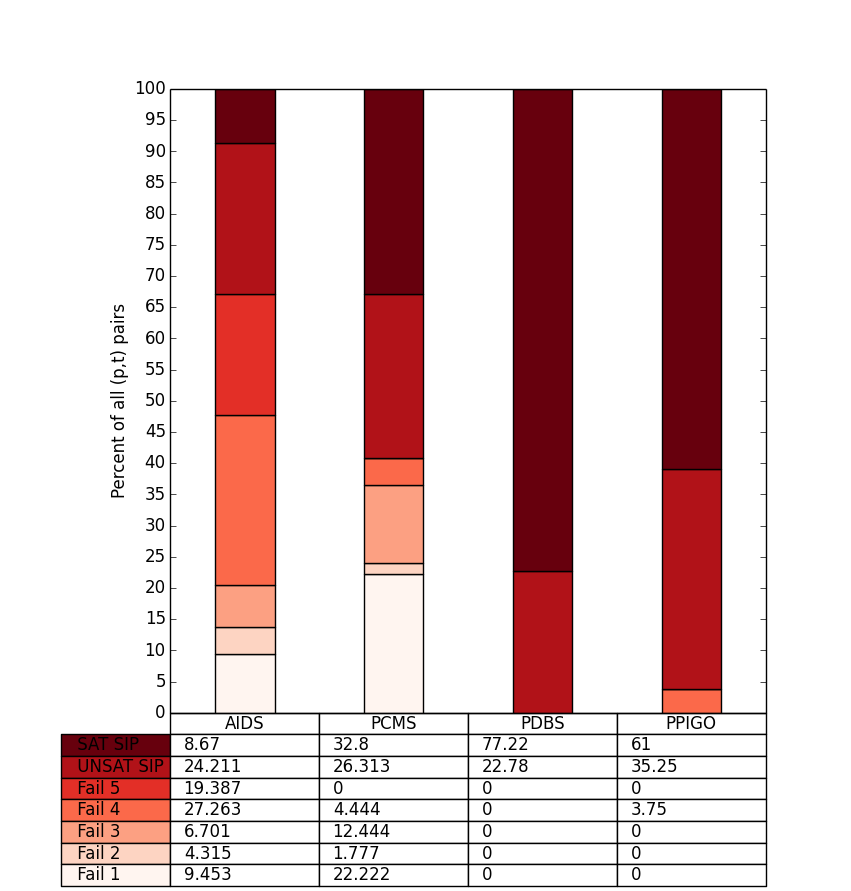
\includegraphics[height=15cm,width=13.5cm]{images/plots/splittedSIP.png}
\caption{Satisifability and average filtering percentage for each method in Table \ref{table:failures} for each of the datasets}
\label{averageFailures}
\end{figure}
%%%

\subsection{Hardness of SIP in terms of search nodes}
We report on the cost of the verification step in terms of the number of \glspl{sn} taken to solve a \gls{sip} instance. A search node denotes the number of recursive \gls{sip} calls taken to find a solution if the problem is \gls{sat} or prove that the problem is \gls{unsat}. For every dataset T, we take all instances that were not rejected during filtering and we compute the number of search nodes taken to solve \gls{sip} for each instance. We then compute the number of instances $|T_i|$ solved in a given number of search nodes $i$ for $0$ $<$ $i$ $<$ $n_{max}$, where  $n_{max}$ is search nodes taken to solve the hardest \gls{sip} instance in T. Figures \ref{aidsNodes}, \ref{pcmsNodes}, \ref{pdbsNodes} and \ref{ppigoNodes} present our results. Here, $|T_i|$ is represented as percentile of all targets (the x-axis). The search effort is plotted, starting from the easiest percentile (the leftmost part of the x-axis) and finishing with the last percentile representing the hardest instances in terms of search effort (on the rightmost part of the x-axis). The y-axis shows the cumulative difficulty of SIP calls in terms of search nodes for each percentile of the targets in a log scale. For example, looking at Figure \ref{aidsNodes}, 24\% of the targets are solved by using at most 2 nodes of search and 50\% of all targets are solved in less than 10 nodes. The hardest instances take at most 600 nodes.

The value on the y-axis for each percentile of T represents the number of search nodes taken to solve the hardest instance that belongs to the percentile. In other words, the graphs below show the hardest instance observed for each percentile of T. For example, if we had 3 graphs that belong to the i$^{th}$ percentile of T and they were solved in 1, 2 and 10 nodes respectively, the y-axis value of i would be 10. Therefore, the datasets are in practice easier than what is shown on Figures \ref{aidsNodes}, \ref{pcmsNodes}, \ref{pdbsNodes} and \ref{ppigoNodes}, which present the hardest instance for each percentile in the dataset. These Figures help us to make the following observations:
\begin{itemize}
\item The easiest dataset is ppigo. Looking at Figure \ref{ppigoNodes}, 88\% of all targets are solved by using at most 4 search nodes, 28\% are solved by using at most 1 node of search effort. The hardest problem (the right-most bar) takes 65 nodes to solve and it is between pattern ``8\_1.6" and target ``\#MUS$/$Mus\_musculus.sif$>$0.5.sif". The time taken to solve this is 4 milliseconds and the instance is \gls{unsat}.

\item pdbs is harder than ppigo and aids with most varied number of search nodes per instance. It is on average harder than pcms, however, the hardest instance in pcms takes more search effort than the hardest instance in pdbs. Figure \ref{pdbsNodes} shows that 20\% of the targets in pdbs are solved by using at most 100 nodes, which is significantly higher than ppigo, where even the hardest instance was solved in less than 70 nodes. The hardest instance here is between pattern ``32$\_$1ARO" and target ``\#g" and it is solved in 7,152 nodes for 95 milliseconds. This instance is \gls{unsat}. 

\item The dataset with the hardest instance is pcms. The hardest SIP takes 10,470 nodes to solve and it is between pattern ``16\_1C5G.cm.A" and target ``1CY2.cm.A.cmap". It was solved in 12 milliseconds and it is unsatisfiable. Looking at the other 99\% of pcms targets, we can see that they are mostly easy. For example, 43\% of the SIP instances are solved by using at most 10 nodes of search effort.

\item The aids dataset is comparably easy. The maximum nodes taken to solve a SIP instance took 619 nodes of search effort. It is the SIP call between pattern \#1 and target \#629591, it took 0 milliseconds of time and it is \gls{unsat}.

\item Looking at aids, pcms and pdbs, the number of nodes taken to solve SIP grows exponentially with the percentile of the population.

\item The hardest instance of each dataset is \gls{unsat}.

\item All four datasets are easy.
\end{itemize}

%%%
\begin{figure}
\centering
\begin{minipage}[t]{.5\textwidth}
  \centering
  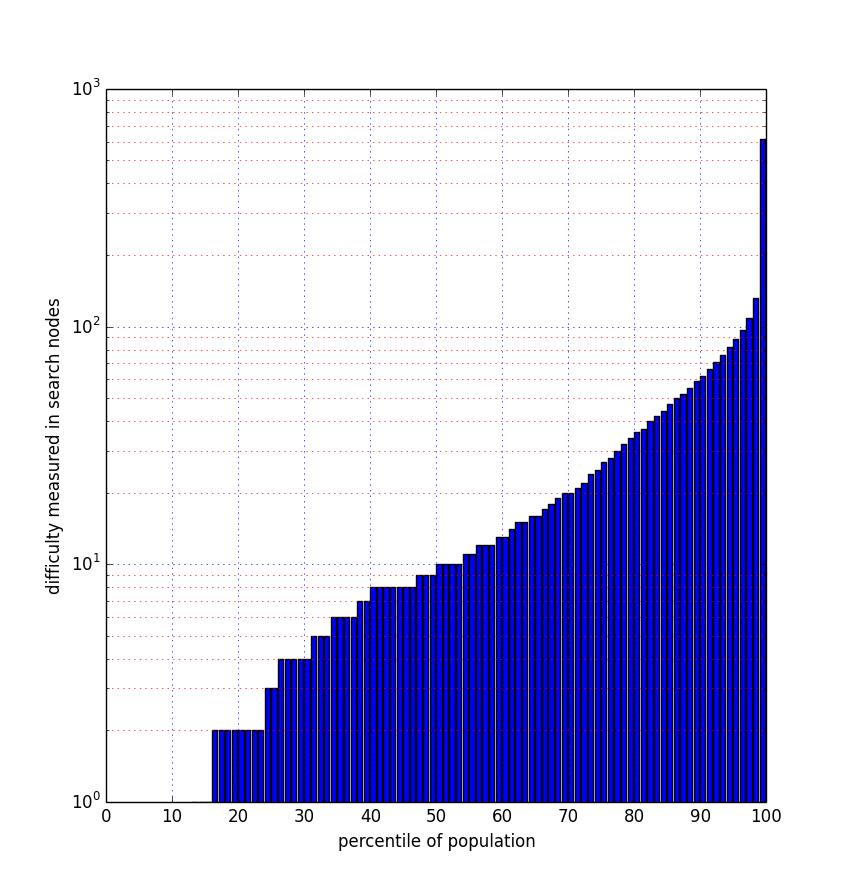
\includegraphics[height=11cm,width=9cm]{images/plots/aidsPercentileLog.png}
  \caption{SIP on aids dataset}
  \label{aidsNodes}
\end{minipage}%
\begin{minipage}[t]{.5\textwidth}
  \centering
  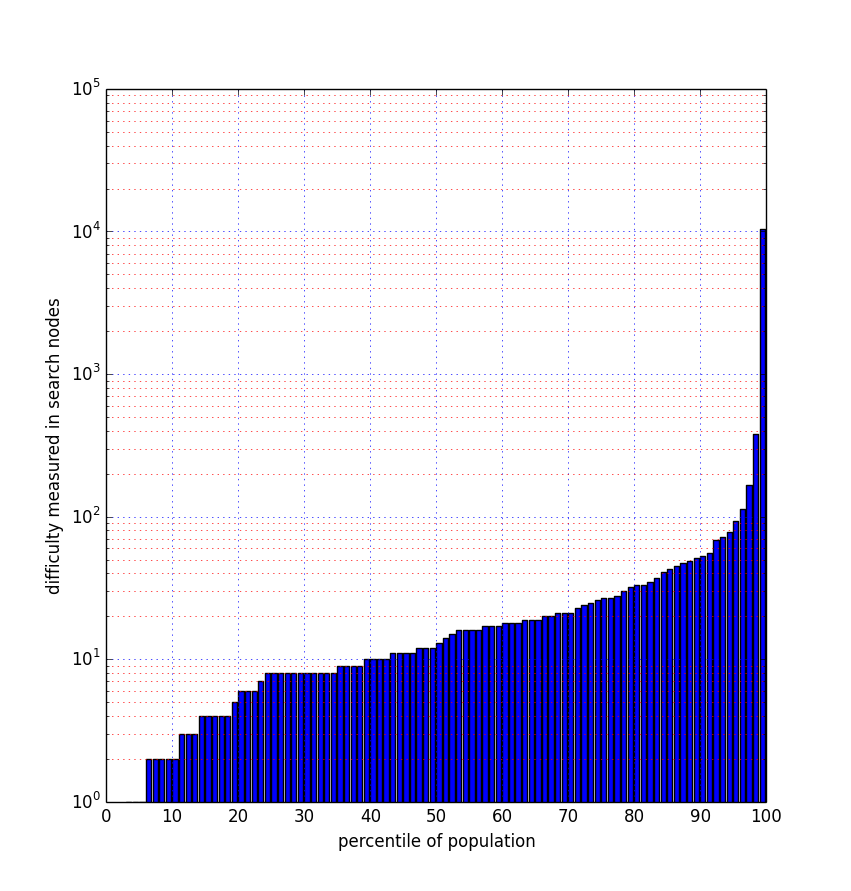
\includegraphics[height=11cm,width=9cm]{images/plots/pcmsPercentileLog.png}
  \caption{SIP on pcms dataset}
  \label{pcmsNodes}
\end{minipage}
\end{figure}
\begin{figure}
\centering
\begin{minipage}[t]{.5\textwidth}
  \centering
  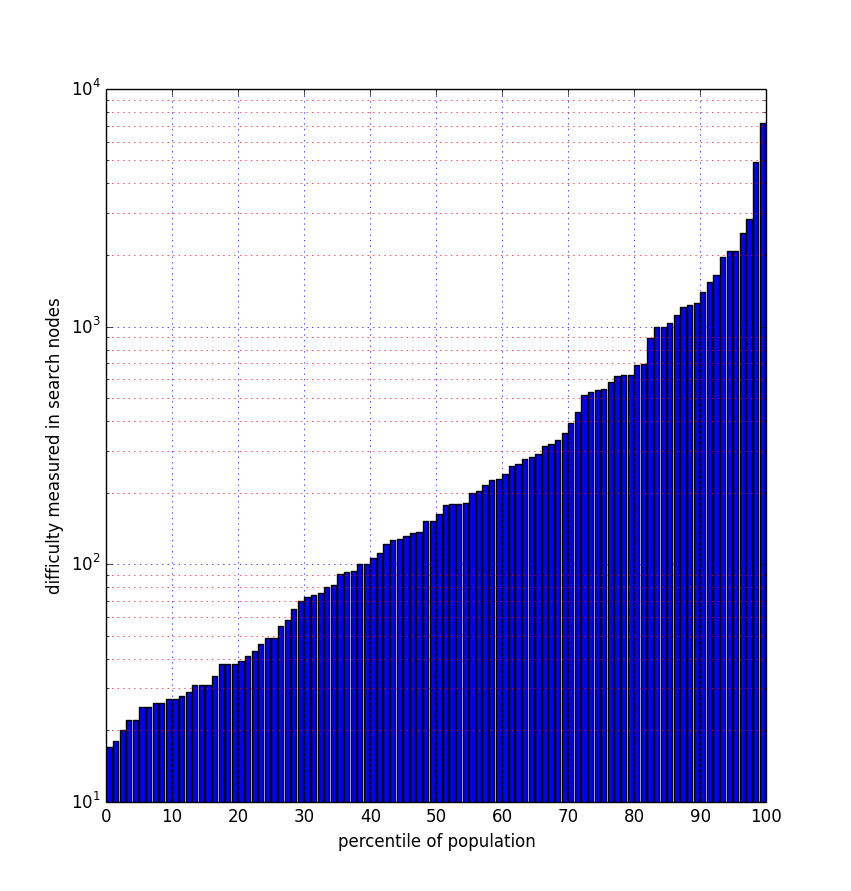
\includegraphics[height=11cm,width=9cm]{images/plots/pdbsPercentileLog.png}
  \caption{SIP on pdbs dataset}
  \label{pdbsNodes}
\end{minipage}%
\begin{minipage}[t]{.5\textwidth}
  \centering
  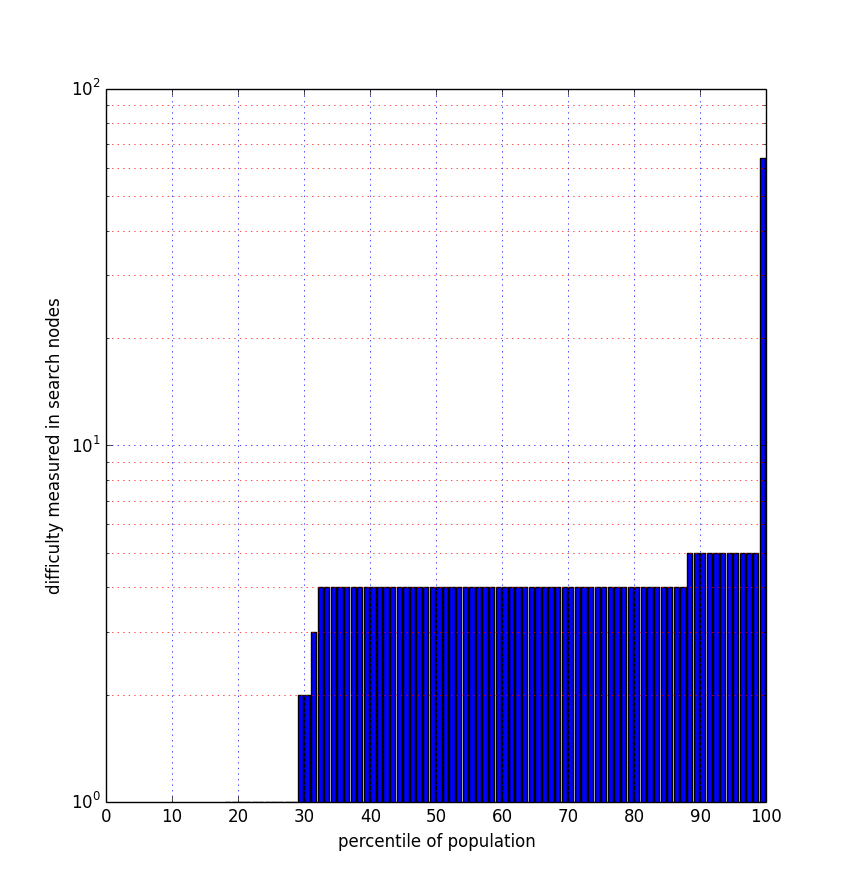
\includegraphics[height=11cm,width=9cm]{images/plots/ppigoPercentileLog.png}
  \caption{SIP on ppigo dataset}
  \label{ppigoNodes}
\end{minipage}
\end{figure}
%%%%

\subsection{Hardness of SAT vs UNSAT SIP instances}

The observation that the hardest instance of each dataset is unsatisfiable raises the following question: is \gls{unsat} \gls{sip} generally harder than SAT SIP? The experiments described in this section are again conducted in terms of number of search nodes and they are intended to further investigate this observation.

The following eight plots below break each of the plots discussed in the previous section (namely \ref{aidsNodes}, \ref{pcmsNodes}, \ref{pdbsNodes} and \ref{ppigoNodes}) further down in terms of whether the SIP instances are \gls{sat} or \gls{unsat}. The blue plots represent all satisfiable SIP pairs for a dataset D. Similarly, the red plots represent all unsatisfiable SIP instances of D. For each D (namely, for aids, pcms, pdbs and ppigo), the union of the blue plot (\gls{sat} \gls{sip}, left-hand side) and the red plot (\gls{unsat} \gls{sip}, right-hand side) gives the plot for the corresponding dataset discussed in the previous Section.

Note that the plots on Figure \ref{fig:ppigoSatUnsat} contain only 4 bars each, i.e. the data is divided into quartiles instead of percentile. Here, each bar represents 25\% of all instances of a category (\gls{sat}/\gls{unsat}). For example, the left plot shows that the lowest quartile of the \gls{sat} \gls{sip} calls takes no more than 4 nodes to solve, as it is also true for the second quartile. We changed the percentile representation for this dataset, because the number of \gls{sat} and \gls{unsat} \gls{sip} (61 and 39 respectively, Table \ref{table:dataSAT}) instances is too small to be scaled to percentiles.
%%% SAT vs UNSAT in terms of search nodes
\begin{figure}
\centering
\begin{minipage}[t]{.5\textwidth}
  \centering
  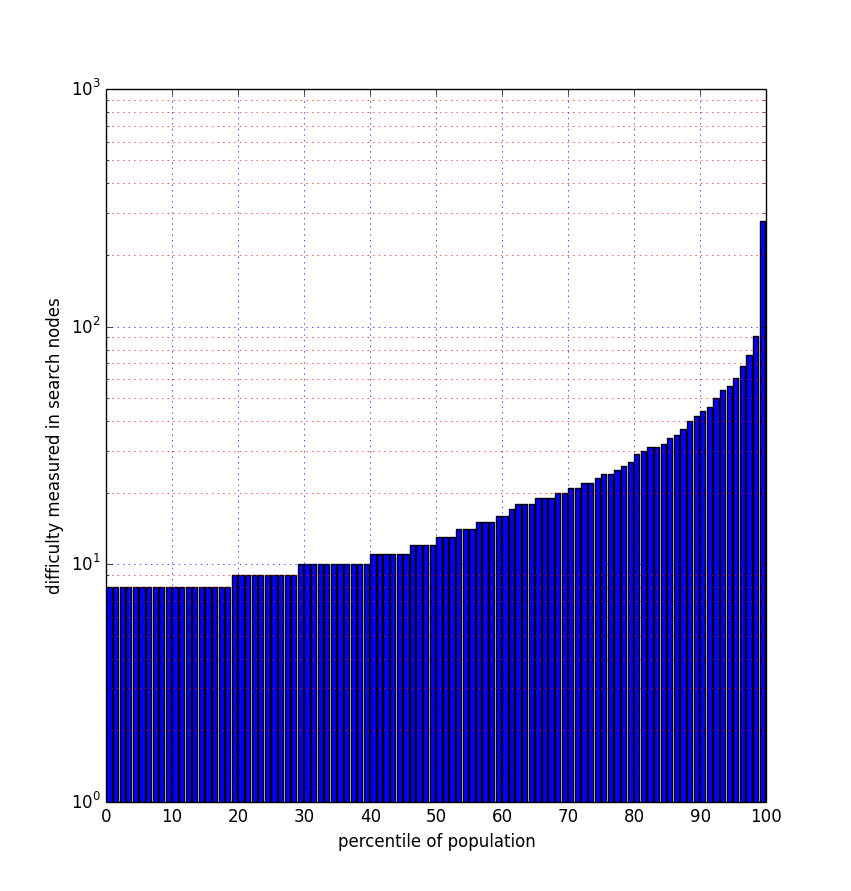
\includegraphics[height=11cm,width=9cm]{images/plots/aidsSAT.png}
\end{minipage}%
\begin{minipage}[t]{.5\textwidth}
  \centering
  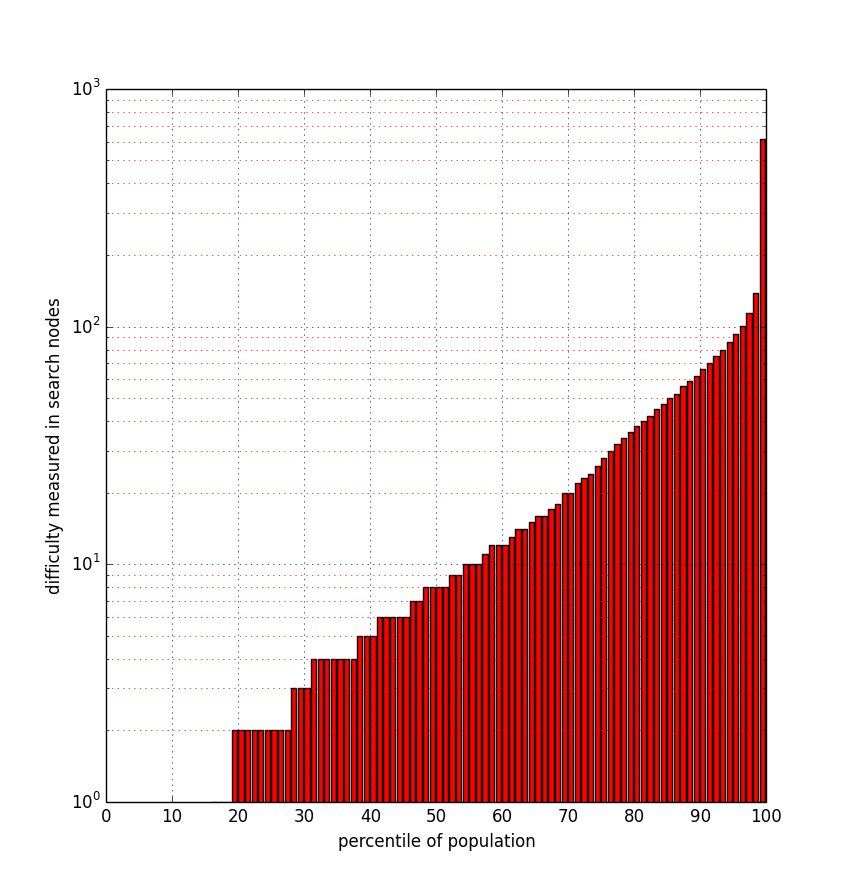
\includegraphics[height=11cm,width=9cm]{images/plots/aidsUNSAT.png}
\end{minipage}
\caption{Search effort for \gls{sat}(blue, left) \gls{unsat}(red, right) \gls{sip} instances in aids}
\label{fig:aidsSatUnsat}
\end{figure}
\begin{figure}
\centering
\begin{minipage}[t]{.5\textwidth}
  \centering
  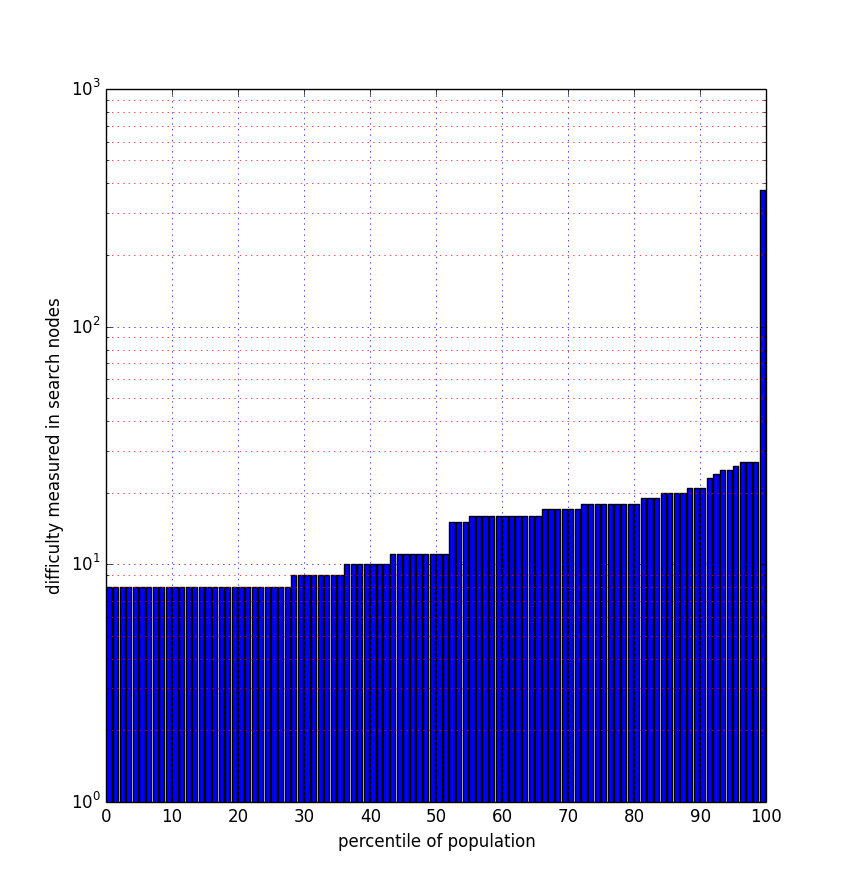
\includegraphics[height=11cm,width=9cm]{images/plots/pcmsSAT.png}
\end{minipage}%
\begin{minipage}[t]{.5\textwidth}
  \centering
  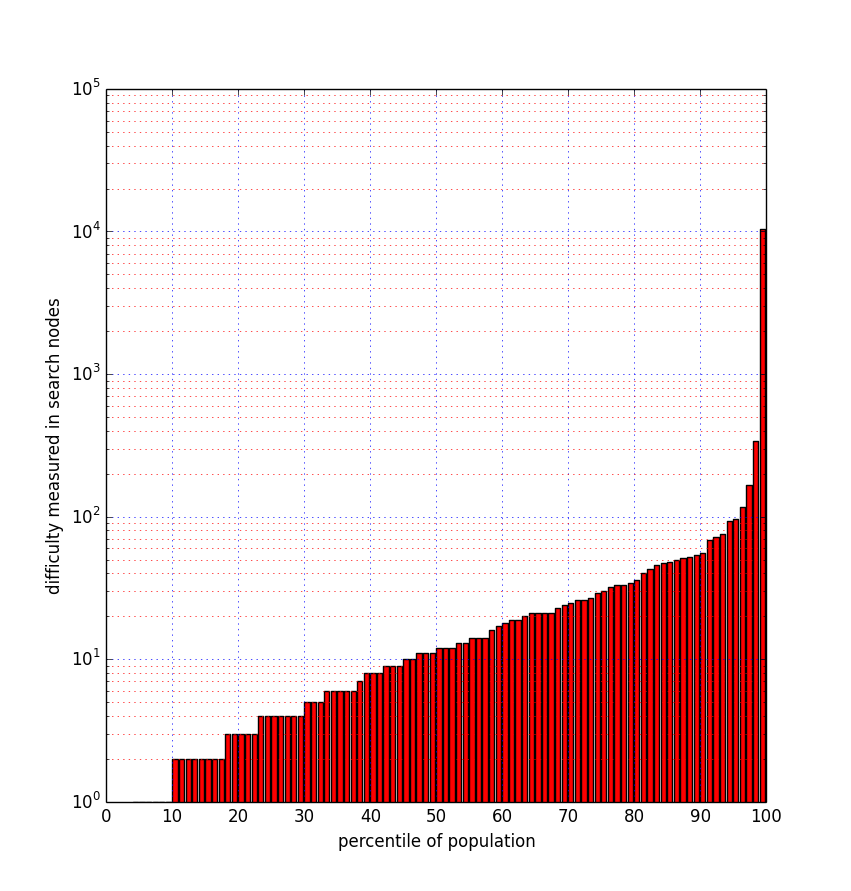
\includegraphics[height=11cm,width=9cm]{images/plots/pcmsUNSAT.png}
\end{minipage}
\caption{Search effort for \gls{sat}(blue, left) \gls{unsat}(red, right) \gls{sip} instances in pcms}
\label{fig:pcmsSatUnsat}
\end{figure}
\begin{figure}
\centering
\begin{minipage}[t]{.5\textwidth}
  \centering
  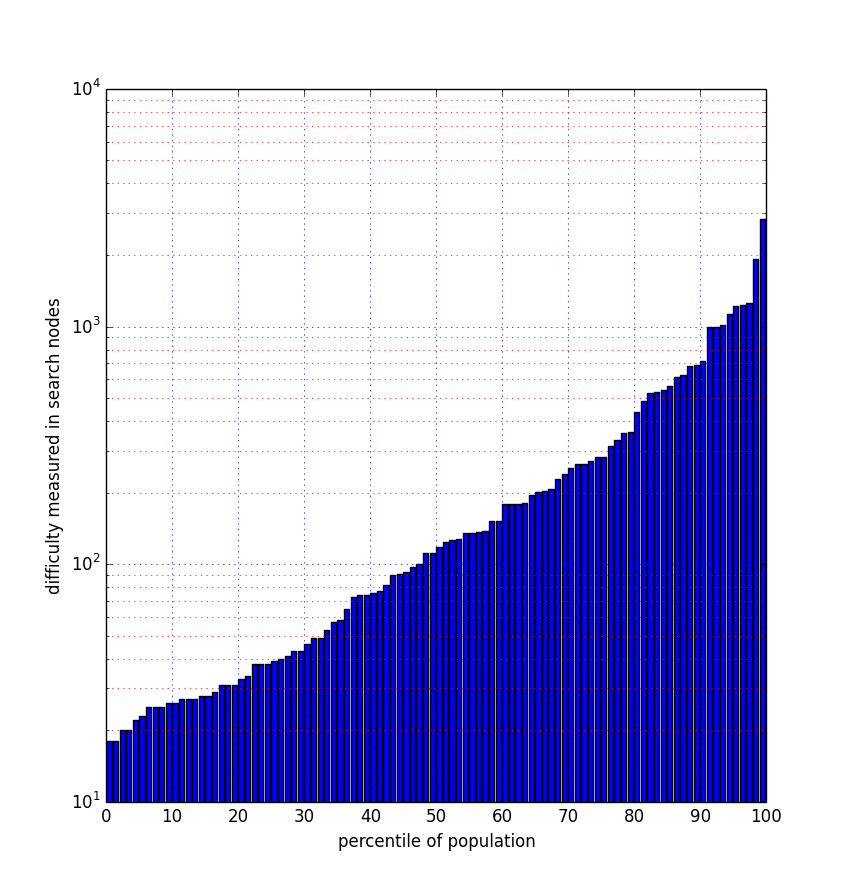
\includegraphics[height=11cm,width=9cm]{images/plots/pdbsSAT.png}
\end{minipage}%
\begin{minipage}[t]{.5\textwidth}
  \centering
  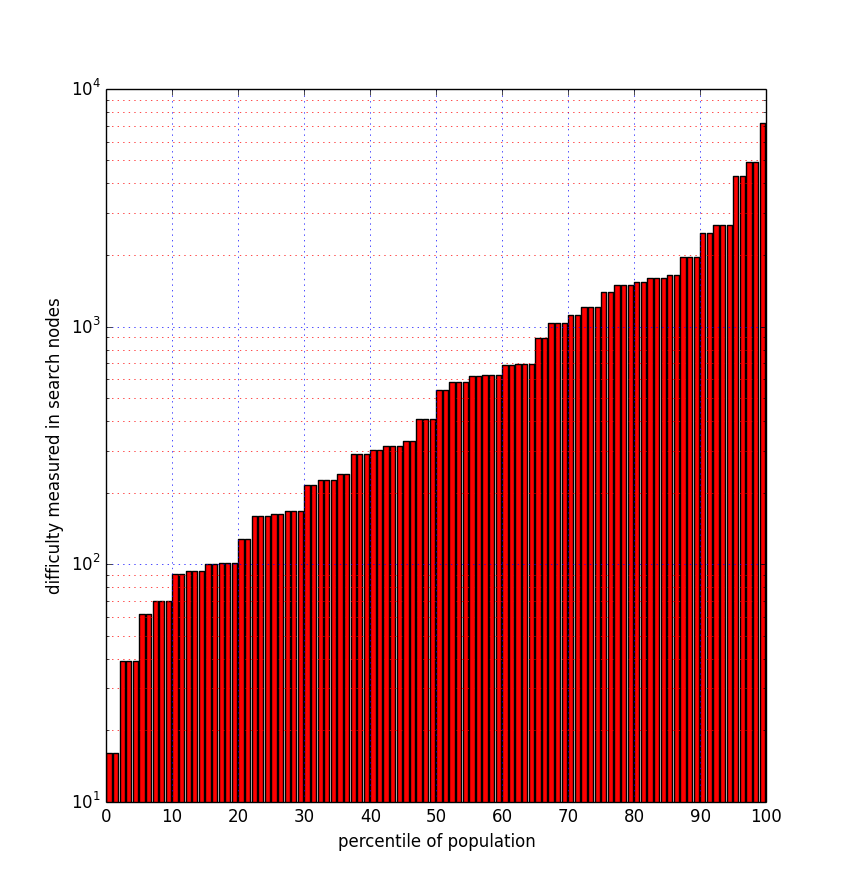
\includegraphics[height=11cm,width=9cm]{images/plots/pdbsUNSAT.png}
\end{minipage}
\caption{Search effort for \gls{sat}(blue, left) \gls{unsat}(red, right) \gls{sip} instances in pdbs}
\label{fig:pdbsSatUnsat}
\end{figure}
\begin{figure}
\centering
\begin{minipage}[t]{.5\textwidth}
  \centering
  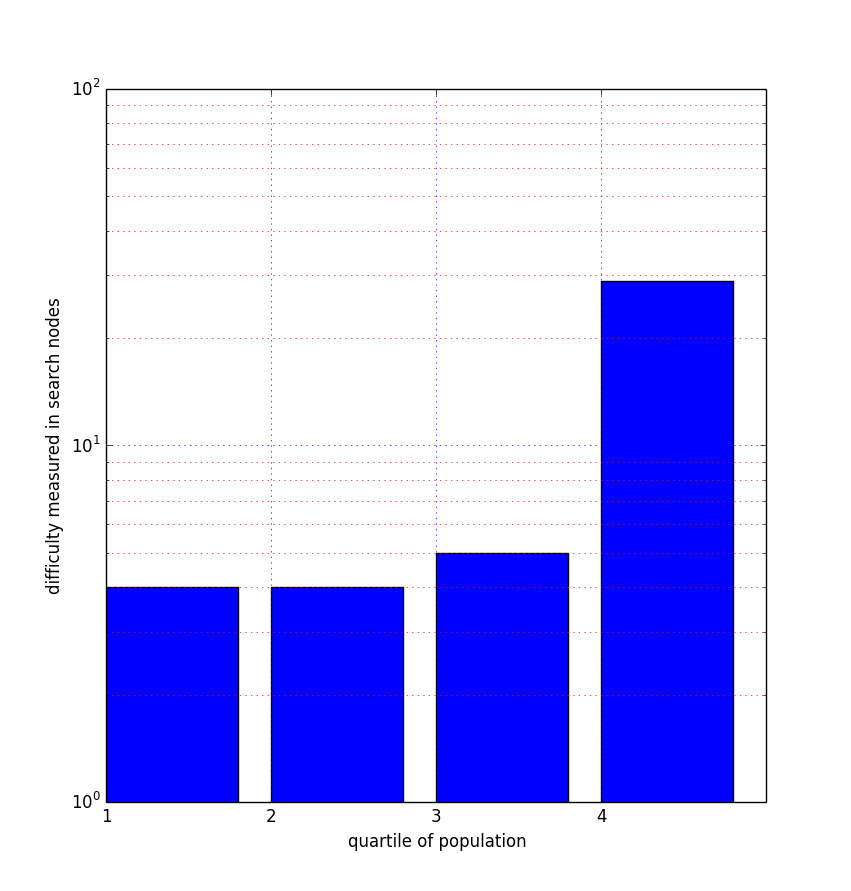
\includegraphics[height=11cm,width=9cm]{images/plots/ppigoSAT.png}
\end{minipage}%
\begin{minipage}[t]{.5\textwidth}
  \centering
  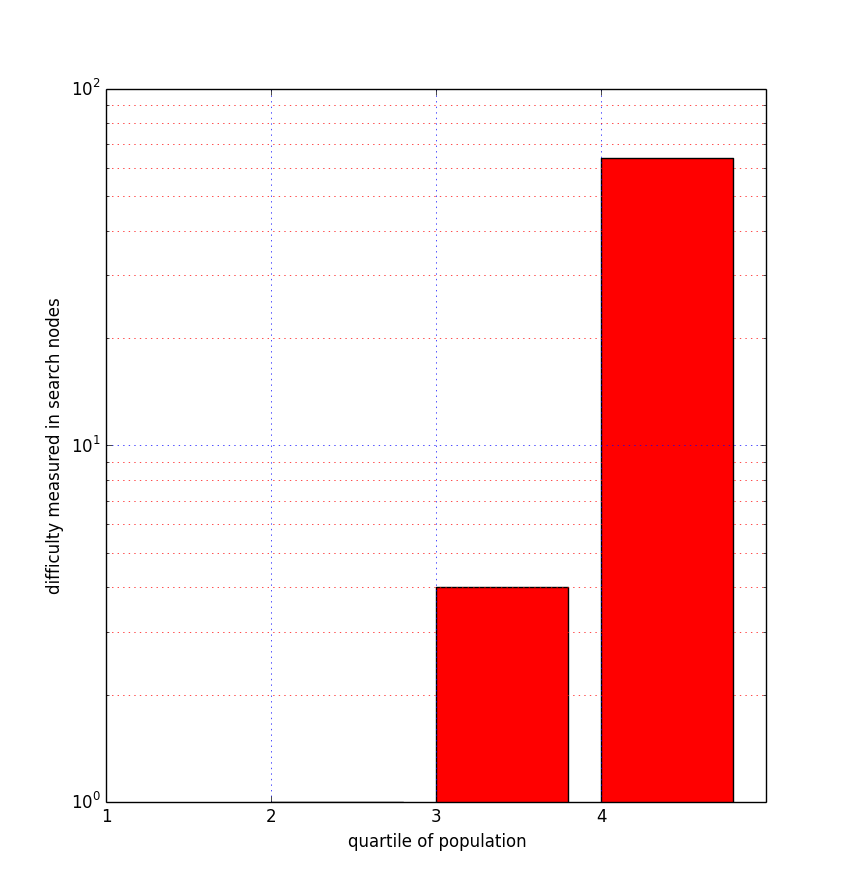
\includegraphics[height=11cm,width=9cm]{images/plots/ppigoUNSAT.png}
\end{minipage}
\caption{Search effort for \gls{sat}(blue, left) \gls{unsat}(red, right) \gls{sip} instances in ppigo}
\label{fig:ppigoSatUnsat}
\end{figure}
%%%%

Table \ref{table:SATUNSATnodes} presents statistics in terms of search effort for \gls{sat} (blue columns) and \gls{unsat} (red columns) instances. For instance, the Table shows that the total number of search nodes taken to solve all \gls{sat} \gls{sip} instances for the aids dataset is 437,108 and the total number of search nodes taken to solve all \gls{unsat} \gls{sip} instances in aids is 2,295,724. Using these Figures, we derive that the total number of search nodes taken to solve all \gls{sip} instances for the aids dataset is the sum of those two numbers, which is equal to 2,732,832. Figure \ref{table:dataSAT} shows the number of instances and percent from each category(SAT/UNSAT). The Table tells us that the reason for the large difference in terms of search effort between SAT and UNSAT instances is that 91\% of all instances are UNSAT (almost ten times more than SAT). Using the Tables and Figures, the following observations can be made:
\begin{itemize}
\item For aids, pcms and ppigo, the easiest percentile of \gls{unsat} \gls{sip} instances require less number of search nodes to be solved than the easiest \gls{sat} \gls{sip} instances. The hardest percentile of \gls{unsat} \gls{sip} take more search effort than the hardest percentile of \gls{sat} \gls{sip} instances.

\item For pdbs, there is a big difference in terms of search effort between SAT and UNSAT problems. For example, \gls{sat} instances are easier for every percentile of the targets (\ref{fig:pdbsSatUnsat}). The tabulated results on Figure \ref{table:SATUNSATnodes} confirm this observation. On average, SAT instances are 3 times easier than UNSAT, the SAT instances median is more than 4 times smaller than the UNSAT instances median and the number of search nodes taken to solve the hardest SAT instance (2,845) is much less than the number of nodes taken to solve the hardest UNSAT instance (7,152).

\item Table \ref{table:SATUNSATnodes} shows that for the pdbs dataset, the total search effort taken to solve unsatisfiable problems is bigger (894,260 nodes taken in total for SAT and 854,720 nodes in total taken for UNSAT problems) contrary to what we observed on the Figures. However, Table \ref{table:dataSAT} shows that \gls{sat} \gls{sip} consists of 77.22\% of all instances in pdbs. Therefore, the large search effort of SAT SIP problems for pdbs is due to their substantially larger number compared to UNSAT problems and in practice, \gls{unsat} \gls{sip} was much more difficult to solve than \gls{sat} \gls{sip} for this dataset. This is confirmed by the average search nodes figures (the second row in Table \ref{table:SATUNSATnodes}), where a SAT instance is on average 3 times easier to solve than an UNSAT instance.

\item The pcms dataset is composed of mostly \gls{unsat} \gls{sip} instances (\ref{table:dataSAT}, \ref{averageFailures}). Similarly to aids, this is the reason why the total number of search nodes for all \gls{unsat} problems is considerably larger than the number of search nodes for all \gls{sat} problems (\ref{table:SATUNSATnodes}). However, the hardest \gls{sat} problem is substantially easier than the hardest \gls{unsat}. The difference is 10,092 search nodes, where the SAT problem takes 378 search nodes to be solved (\ref{table:SATUNSATnodes}) and it is \gls{sip} (``\#32\_1CY1.cm.A.out'', ``\#1CY0.cm.A.cmap''), solved for 4 milliseconds. Average search nodes figures also show that a SAT instance is on average 5 times easier to solve than an UNSAT instance(the second row in Table \ref{table:SATUNSATnodes}).

\item 61\% of all instances in ppigo are \gls{sat} (\ref{table:dataSAT}, \ref{averageFailures}) and this is the main reason why the total SAT SIP search effort is larger than the UNSAT SIP search effort. The average search effort displayed in Table \ref{table:SATUNSATnodes} shows that SAT and UNSAT SIP instances are similarly hard on average for this dataset.
\end{itemize}


\newcolumntype{g}{>{\columncolor{red!15}}r}
\newcolumntype{b}{>{\columncolor{blue!15}}r}
\begin{table}
\centering
        \renewcommand{\arraystretch}{1.5}% Spread rows out...
        \begin{tabular}{c|bg|bg|bg|bg|bg|}
            \cline{2-11}
            &
             \multicolumn{2}{c}{\textbf{Total}} & 
             \multicolumn{2}{|c}{\textbf{Average}} & 
             \multicolumn{2}{|c|}{\textbf{Median}} & 
             \multicolumn{2}{c}{\textbf{Minimum}} & 
             \multicolumn{2}{|c|}{\textbf{Maximum}} \\
              \hline
            \cline{2-11}
             \hline
            % & SAT & UNSAT & SAT & UNSAT & SAT & UNSAT & SAT & UNSAT & SAT & UNSAT\\
            \multicolumn{1}{|c|}{\textbf{aids}}  &437,108  &2,295,724 &21 &10.4   &13  &0   &9  &0  &279   &619 \\
            \multicolumn{1}{|c|}{\textbf{pcms}}  &13,644   &133,276   &23 &110.3  &17  &9   &9  &0  &378   &10,470 \\
            \multicolumn{1}{|c|}{\textbf{pdbs}}  &894,260  &854,720   &322 &1,042.3 &123 &544 &18 &17 &2,845 &7,152 \\
            \multicolumn{1}{|c|}{\textbf{ppigo}} &714      &312       &6.932  &5.8    &6   &2   &5  &0  &30    &65 \\
            \hline
        \end{tabular}
        \caption{Number of nodes of search effort for each dataset. Blue for solvable and red for unsolvable SIP instances}
        \label{table:SATUNSATnodes}
    \end{table}


\subsection{Hardness of SIP in terms of running time}
Table \ref{table:cpuTime} shows the total time in milliseconds taken to solve all \gls{sip} instances of a given dataset. The time on the first row includes file I/O, creating and instantiating objects and domains of variables, the filtering and the verification time. The second row shows the number of milliseconds taken to perform the filtering step and the third: the \gls{sip} algorithm. Note that the filtering step is performed for every sip instance, whereas verification is applied only on instances that were not rejected during filtering. The percentage of calls to sip for each dataset can be seen on Figure \ref{table:failures}.

It is easy to notice that reading in the graphs from a file and instantiating the required objects and variables takes most of the running time for each dataset. For ppigo and pcms, filtering took more time than verification. These figures are very close for the aids dataset (filtering took 2,569 millis. and verification took 2,687 millis.). The 5,006 milliseconds spent on filtering for \gls{sip} problems in pdbs was wasteful, because no instance was rejected (\ref{averageFailures}). Performing \gls{sip} algorithm on all 3,600 instances (\ref{table:dataSAT}) took 16,102 milliseconds, which makes 4.47 milliseconds per instance on average. During the analysis of the search effort, it was noticed that pdbs is the hardest dataset. Achieving so fast verification time shows that the four Big Data datasets are indeed very easy.

\subsubsection{Comparison with Big Data algorithms}
\label{subsubsec:bigDataCompare}
Evaluation of six ``state of the art'' subgraph query processing algorithms (\cite{ctindex,gcode,GRAPES,tree+delta>=graph,graphgrepsx,freqStructBasedIndexing1}) is presented in \cite{foteini}. The algorithms employ a heavy filtering approach using an \gls{index} structure and run \cite{vf2} \gls{sip} algorithm during verification over the \gls{c}. We use the results in this work for comparison with the performance of the light filters method with the evaluated approaches.

In the study described in \cite{foteini}, it was observed that for pcms and ppigo, the filtering stage for four of the evaluated algorithms never finished executing, so the instances never underwent verification. Table \ref{table:cpuTime} shows that the performance of the light filters method is incomparably faster.

For the aids datasets, the fastest of the evaluated algorithms is GraphGrepSX \cite{graphgrepsx} and it took 9 seconds to perform filtering and about 600 milliseconds for verification. It took us 2,569 milliseconds for filtering (\ref{table:cpuTime}), but verification was slower (2,687 milliseconds). The fastest algorithm evaluated in \cite{foteini} took about 7 seconds for filtering and 200 milliseconds for verification and it is again GraphGrepSX \cite{graphgrepsx}. The light filters approach has slower verification and slightly faster filtering.

The algorithms evaluated in \cite{foteini} have an additional overhead that is not present in our approach, which is the size of the index that has to be stored.

TODO: compare with table \ref{table:runningTime} with running times in Section \ref{subsec:ctindexEval}.

\section{Summary of findings}
This Section includes a brief summary of the key points made in this Chapter. 

It was discovered that the Big Data datasets are of poor quality. Two of the datasets have targets that are copied multiple times each. All four datasets contain very easy \gls{sip} instances. The hardest of the datasets is pdbs. Even with the hardest dataset, a \gls{sip} instance took only 4.47 milliseconds to be solved on average. Verification for 50\% of the instances in pdbs took much less than 90 \glspl{sn}, the most expensive \gls{sip} problem costs 10,470 \glspl{sn}. Surprising finding was that the datasets can be easily kept in memory. Big Data is much smaller than what we initially expected. Beneficial future work in this area would be to develop better quality, much bigger and harder datasets. 

Filtering is bound to work only in the area of \gls{unsat} \gls{sip} instances. Consequently, when most of the instances of the dataset are \gls{sat}, filters can be more an overhead than help. The SIP algorithm, performed during verification, can both identify SAT and UNSAT problems. Therefore, constructing sophisticated filtering would give little gain, if any, but implementing fast and smart \gls{sip} would improve the performance significantly.  

We did experiments to find out whether \gls{sat} problems are generally easier than \gls{unsat} problems that were not rejected by filtering. What was observed is that for each of the datasets, the hardest and the easiest instances in terms of \glspl{sn} were \gls{unsat}. Possible way of improvement is to modify the filters algorithm so that it can prune those hard instances. This will involve further investigation of what makes a problem hard. 

\begin{table}
\centering
\renewcommand{\arraystretch}{1.3}% Spread rows out...
\begin{tabular}{ |>{\centering\bfseries}m{1.2in} |>{\centering}m{0.5in}| >{\centering}m{0.5in}| >{\centering}m{0.5in}| >{\centering\arraybackslash}m{0.5in}|} 
\hline
 & \textbf{AIDS} & \textbf{PCMS} & \textbf{PDBS}  & \textbf{PPIGO} \\
\hline
total cpu T & 15,770 & 26,855 & 133,451 & 11,886 \\
\hline
total filtering T & 2,569 & 1,500 & 5,006 & 379 \\
\hline
total verification T & 2,687 & 1,013 & 16,102 & 51 \\
\hline
\end{tabular}
\caption{Total running time in millisec for each dataset}
\label{table:cpuTime}
\end{table}    
   
\chapter{Conclusion and Future work}
	\section{What did we do? What does it suggest?}
    \section{Suggestions for Future work}

%%%%%%%%%%%%%%%%
%              %
%  APPENDICES  %
%              %
%%%%%%%%%%%%%%%%
\begin{appendices}

\chapter{Implementation}

%%%% table with query answers %%%%
\begin{table}[H]
\centering
\renewcommand{\arraystretch}{1.3}% Spread rows out...
\begin{tabular}{ >{\centering\bfseries}m{1in} >{\centering\arraybackslash}m{1.3in}  } 
\toprule
  Query Number & Answers Number\\
\midrule
 \textbf{0} &  8 042\\
 \rowcolor{Gray}
 \textbf{1} & 11 957\\
 \textbf{2} & 78\\
 \rowcolor{Gray}
 \textbf{3} & 461\\
 \textbf{4} & 77\\
  \rowcolor{Gray}
 \textbf{5} & 3\\ 
 \bottomrule
\end{tabular}
\caption{The number of answers for each query for aids dataset}
\label{table:answers}
\end{table}        
%%%%


\begin{table}
\caption{CT-Index: Running time and results}
\label{table:ctindexAllRunningT}
\begin{center}
\begin{tabular}{ |c|p{25mm}|c|c|c|p{18mm}|}\hline
 & fingerprint size \newline max path len\newline max subtree len \newline max cycle len & index build T[sec]& query T[sec]& total T [sec] & \textbf{query\#} \#candidates\TstrutT\Bstrut\\
 \hline
1& 4096 -1 \,5 \,5  & 82.376 & 5.896 & 88.272 & \textbf{0} 11 160 \newline \textbf{1} 13 577 \newline \textbf{2} 975 \newline \textbf{3} 2 950 \newline \textbf{4} 2 575 \newline \textbf{5} 6 \TstrutT\Bstrut\\ 
 \hline
2 & 4096 \,5 \,5 \,\,5 & 108.465  & 5.948 & 114.413 & \textbf{0} 11 168 \newline \textbf{1} 13 589 \newline \textbf{2} 1058 \newline \textbf{3} 2 949 \newline \textbf{4} 2 576 \newline \textbf{5} 6 \TstrutT\Bstrut \\ 
 \hline
3 & 4096 \,5 -1 -1 & 37.621  & 7.929 & 45.550 & \textbf{0} 31 083 \newline \textbf{1} 36 458 \newline \textbf{2} 4 285 \newline \textbf{3} 7 261 \newline \textbf{4} 13 316 \newline \textbf{5} 252 \TstrutT\Bstrut \\ 
 \hline 
4 & 4096 \,5 \,\,1 \,\,1 & 41.482  & 7.96 & 49.442 & \textbf{0} 31 083 \newline \textbf{1} 36 458 \newline \textbf{2} 4 285 \newline \textbf{3} 7 261 \newline \textbf{4} 13 316 \newline \textbf{5} 252 \TstrutT\Bstrut\\ 
 \hline
5 & 2048 \,5 \,\,1 \,\,1 & 41.269  & 13.295 & 54.564 & \textbf{0} 31 085 \newline \textbf{1} 36 458 \newline \textbf{2} 4 293 \newline \textbf{3} 8 539 \newline \textbf{4} 13 319 \newline \textbf{5} 252 \TstrutT\Bstrut\\ 
 \hline
6 &  2048 \,-1 \,\,5 \,\,5 & 87.959  & 8.22 & 96.179 & \textbf{0} 11 540 \newline \textbf{1} 13 582 \newline \textbf{2} 987 \newline \textbf{3} 2 983 \newline \textbf{4} 2 660 \newline \textbf{5} 9 \TstrutT\Bstrut\\ 
 \hline
\end{tabular}
\end{center}
\end{table}
%%%

An example of running from the command line is as follows:
\begin{verbatim}
      > java MaxClique BBMC1 brock200_1.clq 14400
\end{verbatim}
This will apply $BBMC$ with $style = 1$ to the first brock200 DIMACS instance allowing 14400 seconds of cpu time.

\chapter{Generating Random Graphs}
\label{sec:randomGraph}
We generate Erd\'{o}s-R\"{e}nyi random graphs $G(n,p)$ where $n$ is the number of vertices and
each edge is included in the graph with probability $p$ independent from every other edge. It produces
a random graph in DIMACS format with vertices numbered 1 to $n$ inclusive. It can be run from the command line as follows to produce 
a clq file
\begin{verbatim}
      > java RandomGraph 100 0.9 > 100-90-00.clq
\end{verbatim}
\end{appendices}

%%%%%%%%%%%%%%%%%%%%
%   BIBLIOGRAPHY   %
%%%%%%%%%%%%%%%%%%%%

\bibliographystyle{plain}
\bibliography{bib}
\printglossary
\printglossary[type=\acronymtype]
\end{document}
